\documentclass[12pt,a4paper,twoside]{report}
\usepackage[utf8]{inputenc}
\usepackage[T1]{fontenc}
\usepackage[a4paper,inner=30mm,outer=22mm,top=25mm,bottom=25mm,headheight=15pt]{geometry}
\usepackage{setspace}
\usepackage{amsmath,amssymb}
\usepackage{graphicx}
\usepackage[table]{xcolor}
\usepackage{array,longtable,booktabs,tabularx}
\usepackage{caption}
\usepackage{fancyhdr}
\usepackage{enumitem}
\usepackage{listings}
\usepackage{tikz}
\usetikzlibrary{arrows.meta,positioning,shapes.geometric}
\usepackage{xurl}
\usepackage{hyperref}
\usepackage{titlesec}
\usepackage{chngcntr}
\usepackage{ragged2e}
\usepackage{float}
\definecolor{sggreen}{HTML}{176B4D}
\definecolor{sglight}{HTML}{E9F3EE}
\definecolor{sggray}{HTML}{515B55}
\hypersetup{colorlinks=true,linkcolor=sggreen,citecolor=sggreen,urlcolor=sggreen,pdftitle={SchemeGuard Project Report},pdfauthor={Ankesh}}
\setstretch{1.22}
\setlength{\parskip}{0.45em}
\setlength{\parindent}{1.25em}
\setcounter{secnumdepth}{3}
\setcounter{tocdepth}{2}
\counterwithin{figure}{chapter}
\counterwithin{table}{chapter}
\titleformat{\chapter}[display]{\normalfont\bfseries\Huge\filright}{\chaptertitlename\ \thechapter}{1ex}{\titlerule\vspace{1ex}}
\titlespacing*{\chapter}{0pt}{-15pt}{22pt}
\pagestyle{fancy}
\fancyhf{}
\fancyhead[LE]{\small\nouppercase{\leftmark}}
\fancyhead[RO]{\small\nouppercase{\rightmark}}
\fancyfoot[C]{\thepage}
\renewcommand{\headrulewidth}{0.4pt}
\captionsetup{font=small,labelfont=bf}
\lstset{basicstyle=\ttfamily\small,breaklines=true,frame=single,backgroundcolor=\color{sglight},rulecolor=\color{sggreen},columns=fullflexible,keepspaces=true}
\newcommand{\SchemeGuard}{\textsc{SchemeGuard}}
\newcommand{\Unknown}{\textsc{Unknown}}
\newcommand{\StatusNotice}{\textit{SchemeGuard provides informational discovery and assessment demonstrations. It does not make government eligibility decisions or issue official approval.}}
\begin{document}


\begin{titlepage}
\thispagestyle{empty}
\centering
\vspace*{1.3cm}
{\Huge\bfseries\color{sggreen} SCHEMEGUARD\par}
\vspace{0.8cm}
{\Large Personalized Government Scheme Discovery, Evidence-backed Eligibility and Policy Change Monitoring\par}
\vspace{1.2cm}
\IfFileExists{images/SchemeGuard_logo.png}{
\includegraphics[width=0.54\textwidth]{images/SchemeGuard_logo.png}}{%

\begin{tikzpicture}
\draw[sggreen,line width=2pt,rounded corners=10pt] (0,0) -- (0,1.8) -- (1.2,2.2) -- (2.4,1.8) -- (2.4,0.5) -- (1.2,-0.1) -- cycle;
\draw[sggreen,line width=3pt] (0.55,1.05) -- (1.0,0.62) -- (1.85,1.45);
\end{tikzpicture}}
\vspace{1.1cm}

{\Large Project Report\par}
\vspace{0.55cm}
{\large Prepared by\par}
{\Large\bfseries Ankesh\par}
\vspace{0.8cm}
{\large Bachelor of Technology Project\par}
{\large Computer Science and Engineering\par}

\vfill
{\large November 2026\par}
\end{titlepage}

\begin{titlepage}
\thispagestyle{empty}
\centering
\vspace*{1.5cm}
{\Large\bfseries SCHEMEGUARD\par}
\vspace{0.8cm}
{\large Personalized Government Scheme Discovery, Evidence-backed Eligibility and Policy Change Monitoring\par}
\vspace{1.3cm}
{\large A project report submitted in partial fulfilment of the requirements for the degree of\par}
\vspace{0.35cm}
{\Large Bachelor of Technology\par}
{\large in Computer Science and Engineering\par}
\vspace{0.9cm}
{\large by\par}
{\Large\bfseries Ankesh\par}



\vfill
{\large November 2026\par}
\end{titlepage}

\pagenumbering{roman}
\chapter*{Acknowledgement}
\addcontentsline{toc}{chapter}{Acknowledgement}
This project took shape through many rounds of building, testing and reconsidering what the system should claim. I am grateful to the people who tried the application, questioned unclear results and shared feedback that helped make the citizen and administrator journeys easier to understand. I also acknowledge the public departments that maintain the official scheme information used as discovery provenance, and the open-source communities whose tools support the implementation.

The most useful feedback was often a reminder to show uncertainty plainly. That principle shaped the recommendation explanations, the deterministic assessment engine and the document review workflow.

\chapter*{Abstract}
\addcontentsline{toc}{chapter}{Abstract}
\SchemeGuard is a full-stack academic project for personalized discovery of Indian government schemes and traceable assessment of supported requirements. A citizen can share optional profile details and interests to receive explainable, catalog-backed recommendations. The system keeps this relevance ranking separate from eligibility: strict assessments use only applicable, human-approved deterministic rules, preserve source evidence and return \textsc{Pass}, \textsc{Fail} or \textsc{Unknown}. Missing information remains unknown.

The application combines a Next.js interface, FastAPI services, PostgreSQL, immutable document and policy history, PyMuPDF extraction, structured Gemini candidates, a bounded LangGraph review workflow, Celery monitoring and user reassessment. AI output remains pending until an administrator reviews and approves the exact proposed rule revision. Policy updates preserve prior versions and evidence so historical assessments remain reproducible.

The recorded project catalog contains 282 government scheme discovery records, while no government eligibility rule set is approved in the recorded database snapshot. Automated and synthetic integration checks exercise the end-to-end design, but they do not establish current eligibility coverage, real-model accuracy or production deployment. \SchemeGuard is an informational demonstration and does not issue government decisions.

\noindent\textbf{Keywords:} Government schemes, eligibility assessment, evidence provenance, deterministic rules, document processing, policy monitoring, human review.

\tableofcontents
\listoffigures
\listoftables
\clearpage
\pagenumbering{arabic}


\clearpage\chapter{Introduction}

\section{Background}

Indian government programmes span education, agriculture, healthcare, employment, housing and social protection. Information is published through national portals, state directories, ministry pages and policy PDFs. A citizen may find a scheme name without finding the complete, current conditions that apply to an individual application. Scheme discovery and eligibility verification are therefore different engineering problems.

Official services such as myScheme support personalized discovery [1], while departmental guidelines remain the source of policy detail. SchemeGuard is an academic implementation that studies how discovery, document evidence, deterministic evaluation and policy history can be connected responsibly. It does not replace an official application portal or issue government approval.

\section{Motivation}

The project is motivated by three practical needs: reduce manual catalog searching, explain every supported assessment, and preserve what changed when a policy is updated. A useful system must also say when information is missing. Returning UNKNOWN is safer and more accurate than presenting an unsupported positive decision.

\section{Problem Statement}

Given a partially specified citizen profile and a catalog of government scheme metadata, identify schemes worth exploring and explain their relevance. Where an applicable human-approved policy exists, evaluate the supplied information deterministically, retain its supporting evidence and rule version, and identify missing inputs. When an authorized policy document changes, propose and review the change before publishing a new policy and reassessing affected consenting users.

The problem includes uncertainty at several levels: incomplete user information, unknown geographic coverage, inaccessible or image-only documents, ambiguous policy wording, missing effective dates and conflicting versions. None of these uncertainties may be silently converted into a verified eligibility condition.

\section{Objectives}

\begingroup\small\renewcommand{\arraystretch}{1.18}
\begin{longtable}{|>{\RaggedRight\arraybackslash}p{0.2743\textwidth}|>{\RaggedRight\arraybackslash}p{0.6857\textwidth}|}
\caption{Project objectives and measurable completion evidence}\label{tab:project-objectives-and-measurable-completion-evidence}\\
\hline\rowcolor{sglight}\textbf{Objective} & \textbf{Implementation / verification evidence} \\ \hline
\endfirsthead
\caption[]{Project objectives and measurable completion evidence (continued)}\\
\hline\rowcolor{sglight}\textbf{Objective} & \textbf{Implementation / verification evidence} \\ \hline
\endhead
\hline\multicolumn{2}{r}{Continued on next page}\\\endfoot
\hline\endlastfoot
Personalized discovery & Profile-first questionnaire and shared deterministic recommendation service over PostgreSQL. \\ \hline
Explainable assessment & Typed PASS/FAIL/UNKNOWN evaluation with condition traces and missing fields. \\ \hline
Evidence preservation & Immutable document versions, page-aware chunks, located excerpts and source checksums. \\ \hline
Controlled AI processing & Structured Gemini candidates, LangGraph checkpoints and mandatory human publication review. \\ \hline
Policy continuity & Approved-only policy changes, historical replay, consent-aware reassessment and deduplicated notifications. \\ \hline
Reliable engineering & Docker services, incremental migrations, regression tests, isolated demonstration and recovery records. \\ \hline
\end{longtable}
\endgroup\vspace{0.3em}

These objectives describe implemented capabilities; their verification scope and remaining operational gaps are separated in Chapter 5. Broad catalog coverage does not imply equally broad executable policy coverage.

\section{Scope and Limitations}

SchemeGuard supports guest discovery, citizen accounts, optional encrypted profiles, saved approved-policy assessments, an administrator document workspace and selected-source monitoring. The primary journey begins with user preferences rather than a grid of hundreds of records. Manual browsing remains available as a secondary route.

\begingroup\small\renewcommand{\arraystretch}{1.18}
\begin{longtable}{|>{\RaggedRight\arraybackslash}p{0.3106\textwidth}|>{\RaggedRight\arraybackslash}p{0.6494\textwidth}|}
\caption{Recorded dataset and executable-policy scope}\label{tab:recorded-dataset-and-executable-policy-scope}\\
\hline\rowcolor{sglight}\textbf{Item} & \textbf{Recorded status} \\ \hline
\endfirsthead
\caption[]{Recorded dataset and executable-policy scope (continued)}\\
\hline\rowcolor{sglight}\textbf{Item} & \textbf{Recorded status} \\ \hline
\endhead
\hline\multicolumn{2}{r}{Continued on next page}\\\endfoot
\hline\endlastfoot
Government discovery records & 282 identities in 23 category manifests; metadata provenance reviewed. \\ \hline
All database scheme records & 283, including one separate legacy development scheme. \\ \hline
Approved government rule sets & 0; no claim of verified eligibility coverage for 282 schemes. \\ \hline
Approved development rule sets & 1, retained for reproducible demonstrations and historical tests. \\ \hline
Illustrative assessment coverage & 9 project-authored templates cover 225 government metadata records in 14 categories; 57 remain unsupported. \\ \hline
Preserved documents & 2 versions; 1 historical official PDF processed into 4 pages and 26 chunks. \\ \hline
Live monitoring enrollment & 0 sources in the recorded working database; enrollment is deliberate and opt-in. \\ \hline
\end{longtable}
\endgroup\vspace{0.3em}

The illustrative path is explicitly separated from approved government policy. It reuses typed evaluation, but has no government rule citations, is not saved as an approved-policy assessment and cannot trigger policy reassessment. Income and age values from such templates never influence recommendation ranking.

The MVP does not include Aadhaar collection, identity-document processing, payment disbursement, submission to government portals, a large OCR subsystem, email delivery, verified password recovery or production identity verification. Live Gemini accuracy and cloud deployment have not been established.

\section{Organisation of the Report}

Chapter 2 reviews relevant official platforms, retrieval-augmented generation, agent orchestration, structured output and decision/provenance approaches. It identifies the design gap that motivates the project. Chapter 3 formulates discovery and eligibility separately and describes the implemented methodology from metadata intake through policy-change reassessment.

Chapter 4 explains the technology stack, modules, database, API contracts, user interface, security and operational configuration. Chapter 5 reports recorded tests, synthetic workflow outcomes, evaluation counts and local measurements with their limits. Chapter 6 summarizes the contribution and identifies concrete future work. References document external sources and repository evidence. Appendix A records the status of academic integrity reports; Appendix B provides only known author information.

\subsection*{Engineering principles}

The application is a modular monolith with independently running background workers. One canonical document and rule representation is reused across ingestion, human review, monitoring and evaluation. New features append history rather than resetting PostgreSQL or rewriting old decisions. API contracts remain versioned and backward compatible.

Four invariants govern the implementation: only approved applicable policies support strict eligibility decisions; every executable condition requires located evidence; missing information remains UNKNOWN; and an LLM cannot approve a policy or override deterministic output. The demonstration environment labels project-authored material and preserves the distinction between technical tests and genuine government policy approval.

\subsection*{Report evidence boundary}

Counts and test results in this report come from the repository verification snapshot dated 14 November 2026 [14]-[19]. Older phase measurements are identified separately. Preparing this document did not rerun backend tests, publish rules, change user records or deploy services. This boundary makes the report auditable without presenting historical evidence as a new execution.

\clearpage\chapter{Literature Survey}

The survey focuses on approaches relevant to scheme discovery, evidence-grounded document processing and controlled decision automation. It reviews official platforms, research papers and primary technical specifications. Published methods are used as design context; SchemeGuard does not claim to reproduce their benchmark results.

\section{Government Scheme Discovery Platforms}

The Government of India's myScheme initiative describes a service for finding programmes using citizen information and understanding eligibility and application steps [1]. It demonstrates the value of starting with a user's needs. SchemeGuard adopts that interaction direction, while retaining a smaller curated catalog and an explicit academic demonstration scope.

DBT Bharat and the Government of Goa directories provide official scheme identities used in the project's static dataset [2], [3]. Their listings establish traceable discovery metadata, not a complete machine-readable policy. SchemeGuard therefore does not interpret directory presence as an active application window or assume universal state coverage. The National Scholarship Portal is also a provenance source for preserved scholarship records [4].

\section{Retrieval-Augmented Generation}

Lewis et al. introduced retrieval-augmented generation for knowledge-intensive NLP tasks by combining a parametric language model with access to external passages [5]. The work is relevant because policy explanations require identifiable source material rather than reliance on a model's internal memory. Its general retrieval-generation architecture motivates evidence-aware assistance, but it does not by itself establish whether a government clause is current, complete or approved.

SchemeGuard applies a stricter domain boundary: retrieval is scoped to an approved scheme, rule version and exact source document before ranking. Returned passages carry page and checksum references. Similarity can help locate explanatory text, but is never used as a personal eligibility decision. The project does not reproduce the paper's training procedure or its open-domain question-answering benchmarks.

\section{Agent Reasoning and Controlled Workflows}

Yao et al.'s ReAct method interleaves reasoning and actions so that a language model can gather information and revise task execution [6]. It illustrates the usefulness of explicit stages and tool interaction. However, an unrestricted agent is unsuitable for policy activation: a plausible reasoning trace is not proof that a clause has an official source or that a reviewer approved it.

The implementation uses a fixed LangGraph state graph with persisted checkpoints and a human-review interrupt [7]. Its nodes prepare the document, reuse extraction, verify evidence, validate the complete proposal, wait for review, publish or reject, and complete. The graph orchestrates existing services rather than allowing model-generated code or arbitrary actions. LangGraph provides the persistence mechanism; SchemeGuard supplies the authorization and publication invariants.

\section{Structured Document Extraction}

Gemini structured output supports schema-constrained responses and Pydantic-based definitions through the Google GenAI SDK [8]. This reduces formatting ambiguity when requesting candidate fields, typed values, operators and evidence references. A well-formed response can still contain a wrong interpretation, so schema conformance is treated as a technical gate rather than proof of policy truth.

PyMuPDF supports page-level text and block extraction and can assist with table discovery [9]. These capabilities suit digitally generated government PDFs, but reading order and table semantics still require review. SchemeGuard preserves page numbers and source locations; blank, corrupted or image-only pages are marked incomplete instead of filled by the model. A large OCR subsystem is outside the present scope.

\section{Decision Models and Data Provenance}

The Object Management Group's Decision Model and Notation specification formalizes decision descriptions and their inputs [10]. It provides relevant context for separating explicit policy logic from application code. SchemeGuard uses its own bounded typed expression schema; it does not claim DMN or FEEL conformance. Its three-valued outcomes handle missing inputs directly and are independently testable.

The W3C PROV data model distinguishes entities, activities and agents involved in producing information [11]. That perspective is useful for tracing a PDF through extraction, review, publication and assessment. SchemeGuard implements relational provenance with document IDs, page excerpts, revision digests and reviewer references rather than claiming a PROV serialization. The combined design makes evidence lineage and authorized transitions inspectable.

\section{Comparative Summary}

\begingroup\small\renewcommand{\arraystretch}{1.18}
\begin{longtable}{|>{\RaggedRight\arraybackslash}p{0.2296\textwidth}|>{\RaggedRight\arraybackslash}p{0.3130\textwidth}|>{\RaggedRight\arraybackslash}p{0.4174\textwidth}|}
\caption{Related approaches and their relevance to SchemeGuard}\label{tab:related-approaches-and-their-relevance-to-schemeguard}\\
\hline\rowcolor{sglight}\textbf{Source / approach} & \textbf{Useful contribution} & \textbf{Boundary / design response} \\ \hline
\endfirsthead
\caption[]{Related approaches and their relevance to SchemeGuard (continued)}\\
\hline\rowcolor{sglight}\textbf{Source / approach} & \textbf{Useful contribution} & \textbf{Boundary / design response} \\ \hline
\endhead
\hline\multicolumn{3}{r}{Continued on next page}\\\endfoot
\hline\endlastfoot
myScheme [1] & Citizen-oriented scheme discovery and application guidance. & External official platform; SchemeGuard is a separate academic system with a smaller reviewed catalog. \\ \hline
DBT Bharat / Goa [2], [3] & Official, traceable catalog identities and departments. & Directory metadata is not executable eligibility or proof of current enrollment. \\ \hline
Lewis et al., RAG [5] & Retrieve source passages to support language generation. & Scope retrieval to approved versions; citations do not themselves prove policy completeness. \\ \hline
Yao et al., ReAct [6] & Explicit interaction between model reasoning and actions. & Use a bounded graph and authenticated review; models cannot activate policy. \\ \hline
Gemini structured output [8] & Machine-validatable response structures. & Validate semantics, evidence, units and conflicts; candidates stay pending. \\ \hline
DMN / W3C PROV [10], [11] & Explicit decisions and inspectable information lineage. & Custom typed rules and relational provenance; no standards-conformance claim. \\ \hline
\end{longtable}
\endgroup\vspace{0.3em}

The comparison concerns architectural suitability, not a benchmark leaderboard. The reviewed methods solve different tasks and use different datasets, so a single accuracy comparison would be misleading. The project evaluates its own guards, typed decisions and workflow transitions separately in Chapter 5.

\section{Research Gap}

The central gap is the connection between discovery, evidence and change history. A catalog can explain what a programme is without encoding every condition. A generative model can suggest conditions without proving that they are supported. A rule engine can calculate a result while losing the source context or selecting an ambiguous policy version. A monitoring service can detect new bytes without knowing whether eligibility actually changed.

SchemeGuard addresses these gaps through a sequence of accountable boundaries. Relevance matching narrows the catalog using optional profile signals. Official documents remain immutable. Candidate expressions are mapped to a fixed typed language, evidence is located on stored pages, and a reviewer approves an exact saved revision. Eligibility evaluation then uses only the applicable approved version. Later changes append new documents and rules, preserve old reports and trigger authorized reassessment.

\subsection*{Position of the contribution}

The contribution is an integrated engineering design and a reproducible implementation, rather than a newly trained language model or a claim to improve national benefit allocation. The project combines a transparent recommendation heuristic, conservative three-valued logic, version-aware provenance and reliable background execution in one deployable system.

The current limits remain material. No real government rule set has been approved in the working database, broad discovery depends on static metadata, and real Gemini extraction accuracy is unmeasured. The resulting system demonstrates how verified policy support can be added safely; it does not claim completed machine-verifiable coverage for every catalog entry.

\clearpage\chapter{Problem Formulation and Proposed Methodology}

\section{Problem Formulation}

Let S be the catalog of schemes, P a partially specified profile, D the immutable document versions and R the reviewed rule versions. Discovery computes an ordered subset Rec(P, S). Strict eligibility computes E(P, r, t) only when rule r is approved and applicable on assessment date t. A saved assessment retains the exact r, t, minimal inputs and evidence needed to reproduce E.

The outputs belong to different domains: recommendation relevance is HIGH, POTENTIAL or MORE\_INFORMATION, while a deterministic condition result is PASS, FAIL or UNKNOWN. A high relevance score does not establish eligibility. If no approved policy is available, the strict service returns UNKNOWN with no evaluated rule version. Unsupported illustrative assessment requests are also refused rather than fabricated.

A policy change is a reviewed relationship between old and new document/rule versions, not merely a different PDF checksum. Publication and reassessment are separate, auditable activities.

\section{Overview of the Proposed System}

\IfFileExists{images/schemeguard-architecture.png}{\begin{figure}[htbp]\centering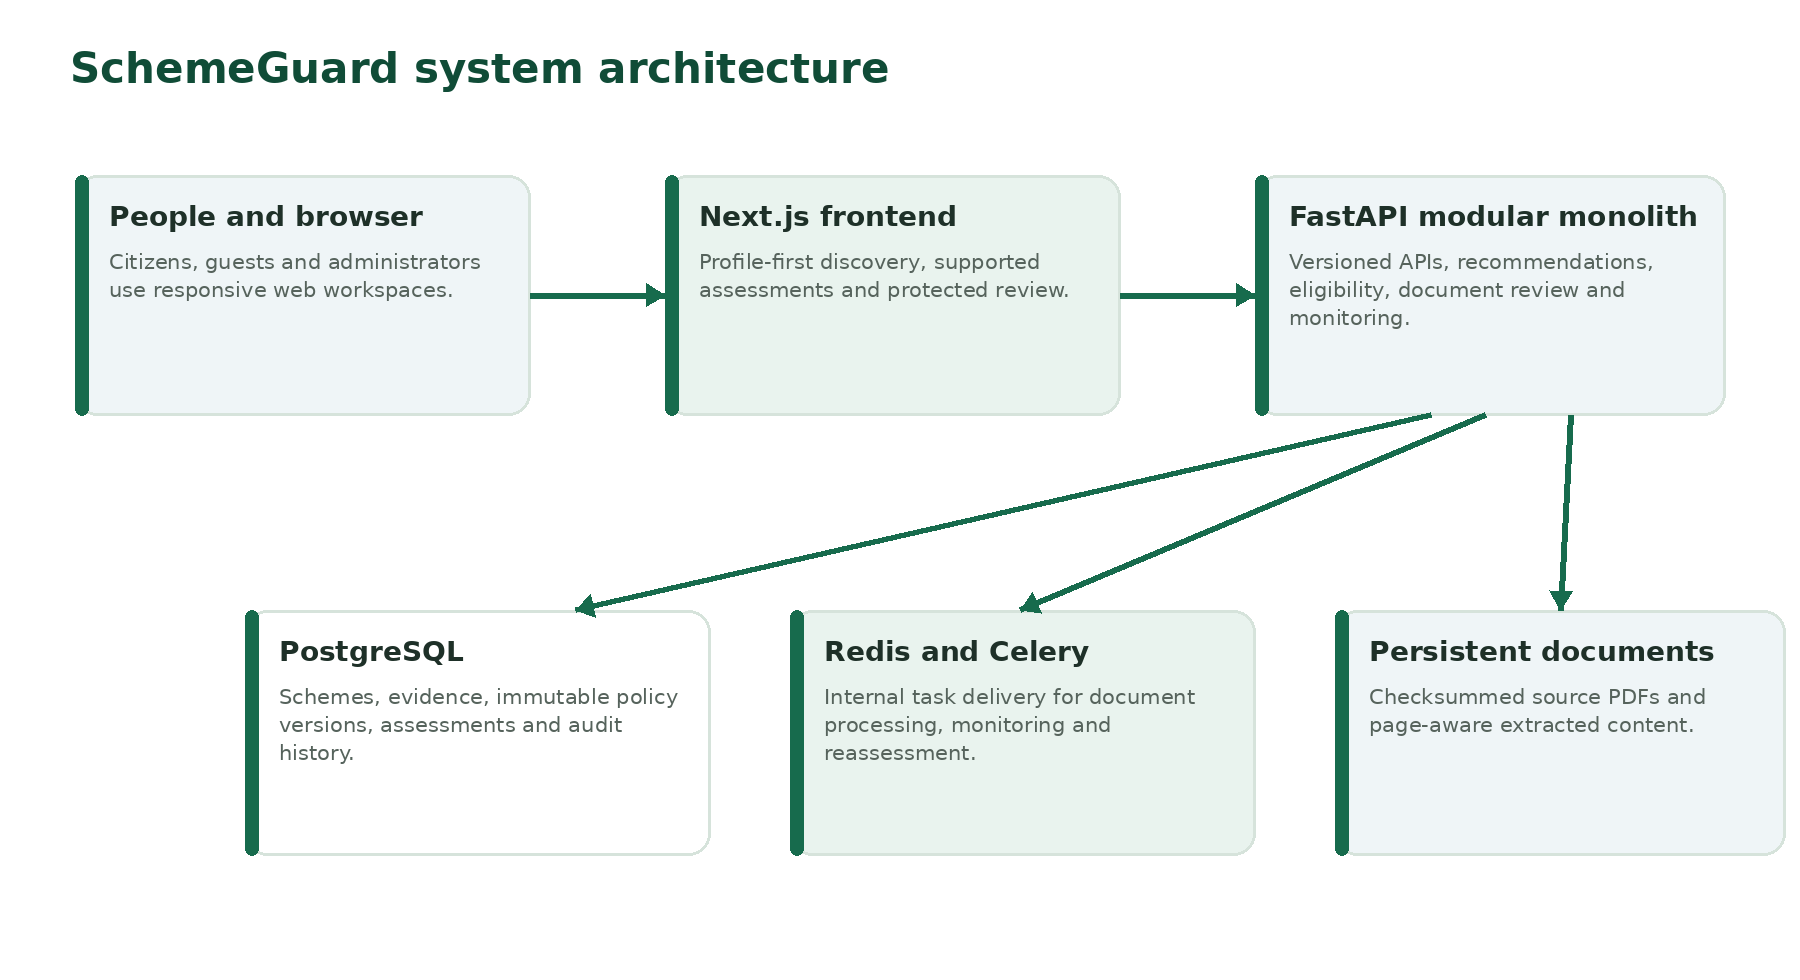
\includegraphics[width=0.94\textwidth,height=0.68\textheight,keepaspectratio]{images/schemeguard-architecture.png}\caption{Overall architecture of SchemeGuard}\label{fig:3-1}\end{figure}}{\begin{figure}[htbp]\centering
\resizebox{0.98\textwidth}{!}{%
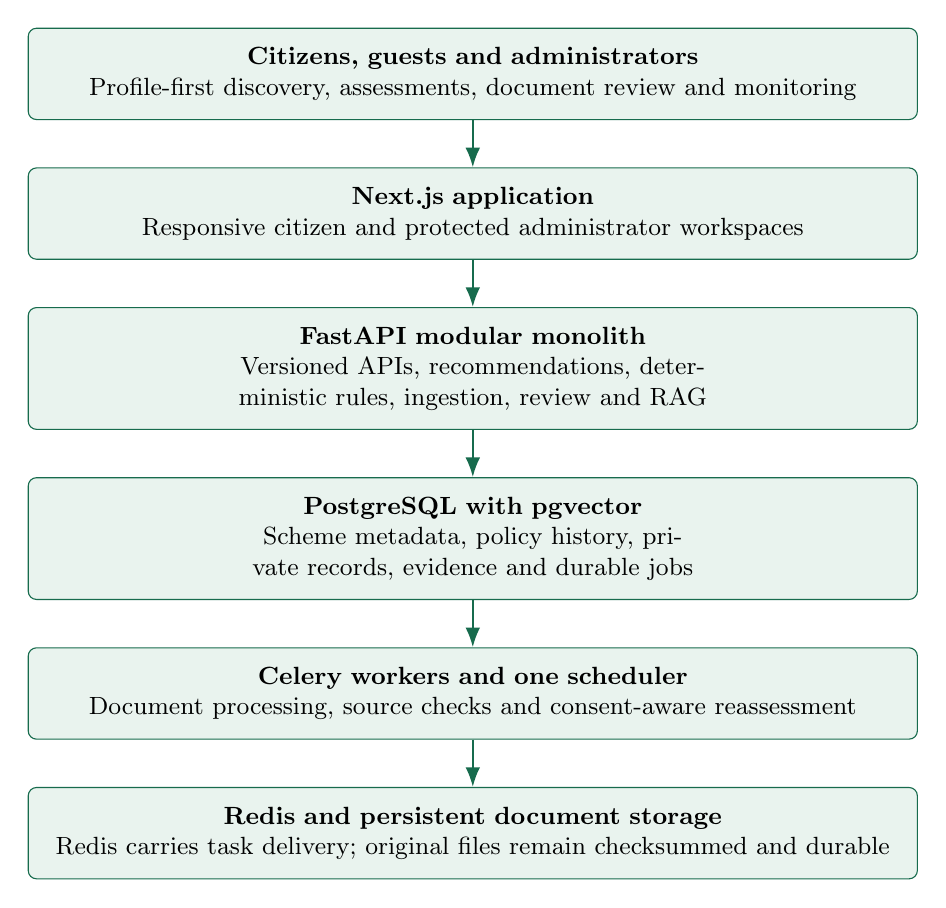
\begin{tikzpicture}[sgbox/.style={draw=sggreen,fill=sglight,rounded corners=3pt,align=center,text width=10.8cm,inner sep=7pt,font=\small},sgarrow/.style={-{Latex[length=2.5mm]},thick,draw=sggreen},node distance=6mm]
\node[sgbox] (people) {\textbf{Citizens, guests and administrators}\\Profile-first discovery, assessments, document review and monitoring};
\node[sgbox,below=of people] (web) {\textbf{Next.js application}\\Responsive citizen and protected administrator workspaces};
\draw[sgarrow] (people.south) -- (web.north);
\node[sgbox,below=of web] (api) {\textbf{FastAPI modular monolith}\\Versioned APIs, recommendations, deterministic rules, ingestion, review and RAG};
\draw[sgarrow] (web.south) -- (api.north);
\node[sgbox,below=of api] (db) {\textbf{PostgreSQL with pgvector}\\Scheme metadata, policy history, private records, evidence and durable jobs};
\draw[sgarrow] (api.south) -- (db.north);
\node[sgbox,below=of db] (jobs) {\textbf{Celery workers and one scheduler}\\Document processing, source checks and consent-aware reassessment};
\draw[sgarrow] (db.south) -- (jobs.north);
\node[sgbox,below=of jobs] (infra) {\textbf{Redis and persistent document storage}\\Redis carries task delivery; original files remain checksummed and durable};
\draw[sgarrow] (jobs.south) -- (infra.north);
\end{tikzpicture}%
}\caption{Overall architecture of SchemeGuard}\label{fig:3-1}\end{figure}}

The frontend provides guest, citizen and administrator experiences. FastAPI exposes versioned contracts and delegates to reusable services. PostgreSQL stores authoritative scheme metadata, immutable policy history, encrypted private records, durable jobs and graph checkpoints. Workers run the same ingestion and evaluation services independently from request handling.

The document path and the citizen path meet only at approved policy versions and source-grounded reports. Applicant profiles are not sent to Gemini or embedded for RAG. Redis is a delivery mechanism for job identifiers, while original documents live in persistent storage with checksummed references. This separation prevents a model response or broker message from becoming the authoritative policy record.

\section{Data Collection and Pre-processing}

The static catalog is organized as 23 category JSON manifests. The expansion preserved the original five scholarship records and added 277 distinct government identities: 224 central directory records and 53 Goa state records [14]. Every record has a stable slug, source provenance and a verification date. Unverified geography, benefits, thresholds and deadlines remain unknown.

\begingroup\small\renewcommand{\arraystretch}{1.18}
\begin{longtable}{|>{\RaggedRight\arraybackslash}p{0.3020\textwidth}|>{\RaggedRight\arraybackslash}p{0.1187\textwidth}|>{\RaggedRight\arraybackslash}p{0.5393\textwidth}|}
\caption{Catalog provenance and verification scope}\label{tab:catalog-provenance-and-verification-scope}\\
\hline\rowcolor{sglight}\textbf{Source group} & \textbf{Records} & \textbf{What was verified} \\ \hline
\endfirsthead
\caption[]{Catalog provenance and verification scope (continued)}\\
\hline\rowcolor{sglight}\textbf{Source group} & \textbf{Records} & \textbf{What was verified} \\ \hline
\endhead
\hline\multicolumn{3}{r}{Continued on next page}\\\endfoot
\hline\endlastfoot
Original official scholarship sources & 5 & Preserved metadata and original source relationships; review date 11 November 2026. \\ \hline
DBT Bharat central directory & 224 new & Named entries and departmental context, reviewed 12 November 2026. \\ \hline
Government of Goa directory & 53 new & Distinct state-programme identities and listed source references, reviewed 12 November 2026. \\ \hline
Government catalog total & 282 & Identity and discovery metadata; not complete current policy eligibility. \\ \hline
\end{longtable}
\endgroup\vspace{0.3em}

The loader validates every manifest before importing. It rejects unsupported properties, category mismatches, duplicate slugs, normalized duplicate names, unsafe official URLs and inconsistent state applicability. A transaction-scoped advisory lock serializes insertion. Existing slugs are skipped without rewriting their UUIDs, sources or historical rules; a failure rolls back the import.

\subsection*{Document pre-processing}

Authorized originals are hashed and registered before extraction. Text normalization is conservative: it supports locating excerpts and comparing content but does not invent a missing clause. Page text, blocks, extraction issues and chunk identities are retained so that reviewers can return to the source. Policy publication dates are not inferred from download timestamps or PDF metadata.

\section{Explainable Profile-based Recommendations}

Recommendation inputs reuse the existing optional ProfileData schema. Interests map to the catalog taxonomy; occupation, employment and explicit student status add broad relevance signals. Verified geography can refine a result, while unknown coverage remains included with an explanation. Only an explicitly verified state mismatch can exclude a geographically incompatible record.

\begingroup\small\renewcommand{\arraystretch}{1.18}
\begin{longtable}{|>{\RaggedRight\arraybackslash}p{0.4000\textwidth}|>{\RaggedRight\arraybackslash}p{0.1200\textwidth}|>{\RaggedRight\arraybackslash}p{0.4400\textwidth}|}
\caption{Implemented additive relevance factors}\label{tab:implemented-additive-relevance-factors}\\
\hline\rowcolor{sglight}\textbf{Signal} & \textbf{Points} & \textbf{Interpretation} \\ \hline
\endfirsthead
\caption[]{Implemented additive relevance factors (continued)}\\
\hline\rowcolor{sglight}\textbf{Signal} & \textbf{Points} & \textbf{Interpretation} \\ \hline
\endhead
\hline\multicolumn{3}{r}{Continued on next page}\\\endfoot
\hline\endlastfoot
Selected interest matches category & +60 & Project-authored relevance heuristic. \\ \hline
Occupation / employment category match & +20 once & Explicit input signal, not inferred demographics. \\ \hline
Current student and education category & +20 & Broad educational relevance. \\ \hline
Verified national / matching-state coverage & +8 & Catalog provenance supports applicability. \\ \hline
Safely loadable approved assessment & +5 & Reviewed policy is available. \\ \hline
Positive direct approved education match & +15 & Conservative typed approved-condition comparison. \\ \hline
All known approved conditions pass & +12 & Existing deterministic engine result. \\ \hline
Known approved conditions fail & -20 & Visible warning; never hidden as a score alone. \\ \hline
\end{longtable}
\endgroup\vspace{0.3em}

Ranking uses the sum of applicable factors, with a HIGH label at 75 points or above. Other matches are POTENTIAL; a reviewed-condition failure is labeled MORE\_INFORMATION with a warning. At least one substantive profile/category or approved-condition signal is required. Geography and assessment availability alone cannot recommend an unrelated scheme.

Tie-breaking is deterministic by case-insensitive scheme name and UUID. Category filters apply to the matched set before pagination. Scores are ordering heuristics, not confidence percentages. Illustrative income/age thresholds never enter this ranking function.

\section{Deterministic Eligibility Evaluation}

The engine evaluates a validated abstract syntax tree. Comparisons support ==, !=, \textgreater{}, \textless{}, \textgreater{}=, \textless{}=, IN and NOT IN over declared number, string, boolean and ISO-date values. Decimal normalization avoids inconsistent financial boundary comparisons. No stored expression is executed as Python code; eval() and exec() are not used.

\begingroup\small\renewcommand{\arraystretch}{1.18}
\begin{longtable}{|>{\RaggedRight\arraybackslash}p{0.2133\textwidth}|>{\RaggedRight\arraybackslash}p{0.2133\textwidth}|>{\RaggedRight\arraybackslash}p{0.2667\textwidth}|>{\RaggedRight\arraybackslash}p{0.2667\textwidth}|}
\caption{Three-valued AND and OR semantics}\label{tab:three-valued-and-and-or-semantics}\\
\hline\rowcolor{sglight}\textbf{A} & \textbf{B} & \textbf{AND(A, B)} & \textbf{OR(A, B)} \\ \hline
\endfirsthead
\caption[]{Three-valued AND and OR semantics (continued)}\\
\hline\rowcolor{sglight}\textbf{A} & \textbf{B} & \textbf{AND(A, B)} & \textbf{OR(A, B)} \\ \hline
\endhead
\hline\multicolumn{4}{r}{Continued on next page}\\\endfoot
\hline\endlastfoot
PASS & PASS & PASS & PASS \\ \hline
PASS & FAIL & FAIL & PASS \\ \hline
PASS & UNKNOWN & UNKNOWN & PASS \\ \hline
FAIL & FAIL & FAIL & FAIL \\ \hline
FAIL & UNKNOWN & FAIL & UNKNOWN \\ \hline
UNKNOWN & UNKNOWN & UNKNOWN & UNKNOWN \\ \hline
\end{longtable}
\endgroup\vspace{0.3em}

For groups of any supported size, AND returns FAIL if any child fails; otherwise UNKNOWN if any child is unknown; otherwise PASS. OR returns PASS if any child passes; otherwise UNKNOWN if any child is unknown; otherwise FAIL. These rules preserve incomplete information instead of treating absence as success.

Exclusions invert established truth: a matching exclusion produces FAIL, a nonmatching exclusion produces PASS, and an unknown exclusion stays UNKNOWN. A conditional evaluates its guard first. An unknown prerequisite keeps the conditional UNKNOWN; a known guard selects only the applicable branch. Missing fields in irrelevant branches are not demanded as established requirements.

Every node produces a stable key, label, result, explanation, missing fields and child traces. The report presents these as known conditions satisfied, requirements not satisfied or more information required. None of the labels constitutes government approval.

\subsection*{Typed example and version gate}

The following expression is a \textbf{fictional test clause}, used only to explain the data shape. The value is not asserted as the threshold of any real government scheme.

For this test clause, an input of 250000 passes the inclusive boundary; 250001 fails; an absent or null income produces UNKNOWN. The boundary is fixed by the stored operator and typed value. A language model is not called during evaluation.

Before the engine runs, the eligibility service loads a policy through the approved-version repository. Draft, rejected, future or expired policies cannot support the current decision. Unrelated overlapping applicable versions raise a conflict instead of silently choosing the largest number. A reviewed replacement relationship can resolve an overlap while preserving prior content.

Program validation rejects duplicate expression keys, references to undeclared fields, incompatible operators and types, non-finite numbers, malformed dates and oversized trees. The implementation bounds depth to 12, total nodes to 128 and program inputs to 32 fields. These limits constrain both accidental complexity and malicious stored input.

The strict policy service remains distinct from the opt-in illustrative assessment path. A server-selected criteria token prevents a stale questionnaire from silently evaluating against a changed basis. Illustrative output includes its template version and fingerprint, no approved RuleSet and no supporting government rule citations. Such output is transient and is not written into policy assessment history.

\section{Secure PDF Ingestion and Chunking}

\IfFileExists{images/document-processing-workflow.png}{\begin{figure}[htbp]\centering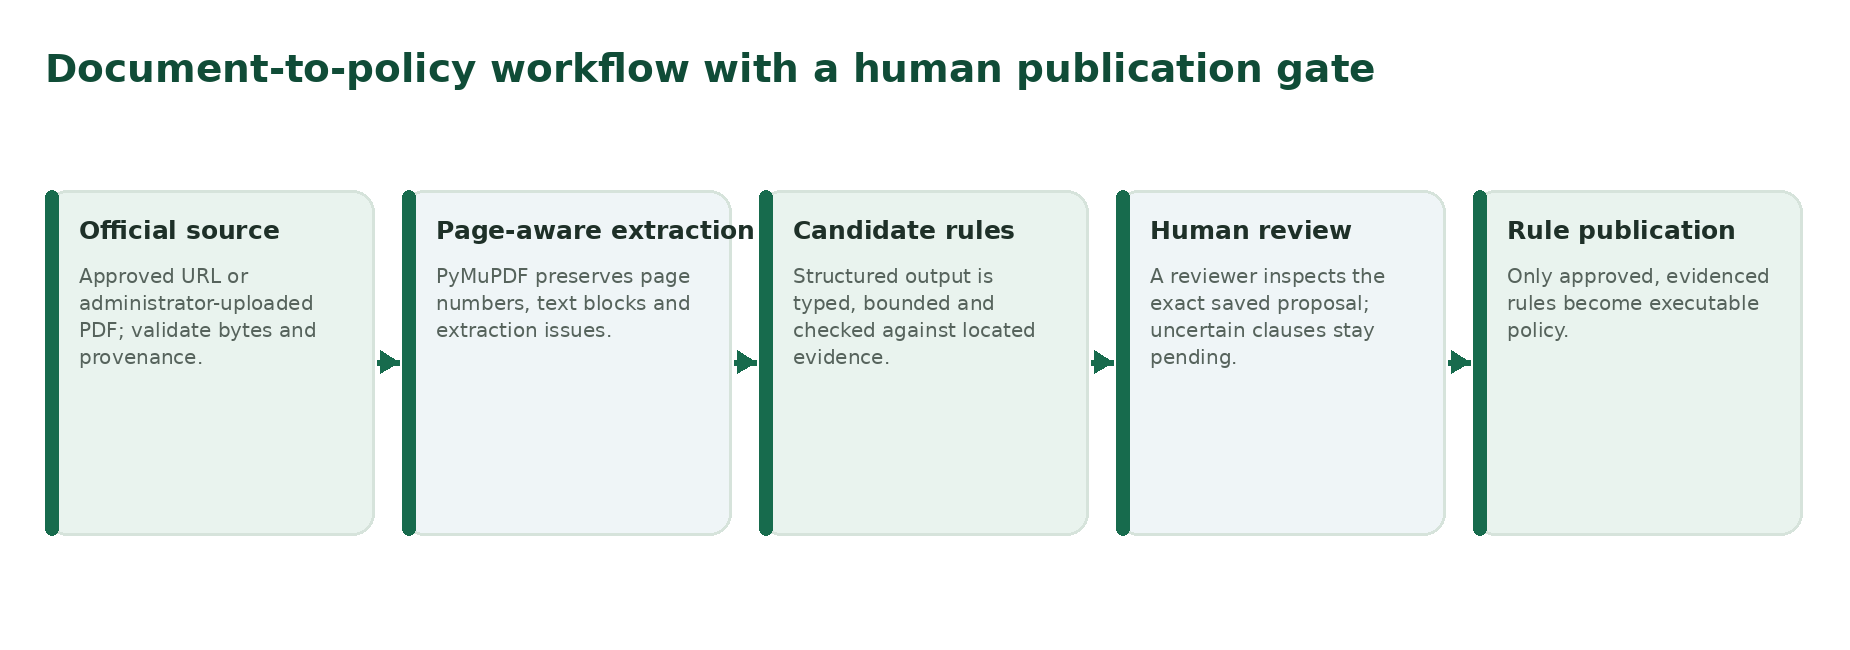
\includegraphics[width=0.94\textwidth,height=0.68\textheight,keepaspectratio]{images/document-processing-workflow.png}\caption{Document-to-policy workflow with a human publication gate}\label{fig:3-2}\end{figure}}{\begin{figure}[htbp]\centering
\resizebox{0.98\textwidth}{!}{%
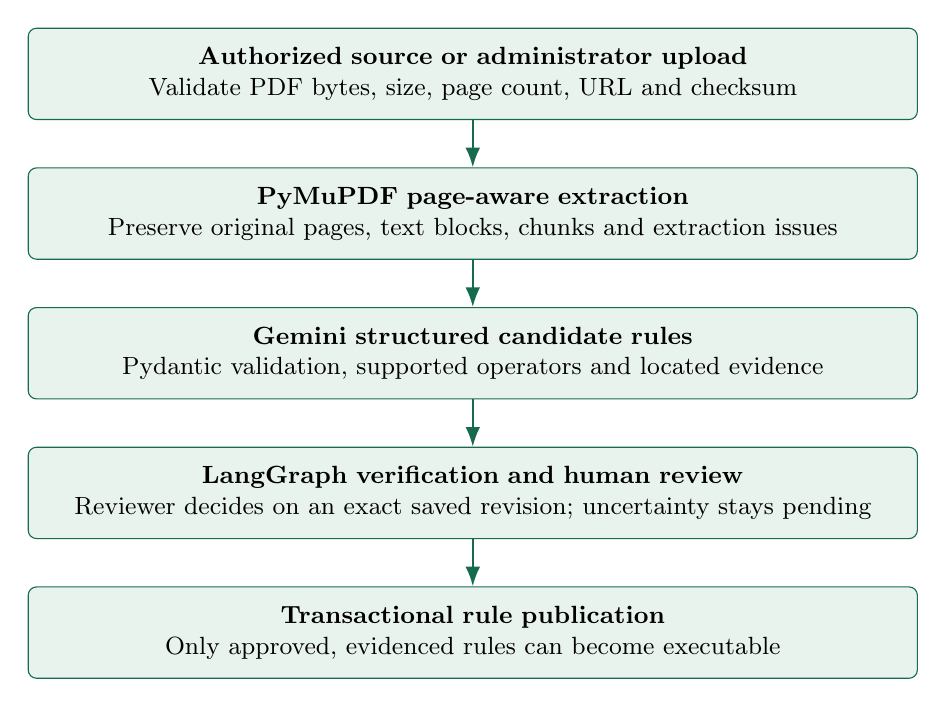
\begin{tikzpicture}[sgbox/.style={draw=sggreen,fill=sglight,rounded corners=3pt,align=center,text width=10.8cm,inner sep=7pt,font=\small},sgarrow/.style={-{Latex[length=2.5mm]},thick,draw=sggreen},node distance=6mm]
\node[sgbox] (n1) {\textbf{Authorized source or administrator upload}\\Validate PDF bytes, size, page count, URL and checksum};
\node[sgbox,below=of n1] (n2) {\textbf{PyMuPDF page-aware extraction}\\Preserve original pages, text blocks, chunks and extraction issues};
\draw[sgarrow] (n1.south) -- (n2.north);
\node[sgbox,below=of n2] (n3) {\textbf{Gemini structured candidate rules}\\Pydantic validation, supported operators and located evidence};
\draw[sgarrow] (n2.south) -- (n3.north);
\node[sgbox,below=of n3] (n4) {\textbf{LangGraph verification and human review}\\Reviewer decides on an exact saved revision; uncertainty stays pending};
\draw[sgarrow] (n3.south) -- (n4.north);
\node[sgbox,below=of n4] (n5) {\textbf{Transactional rule publication}\\Only approved, evidenced rules can become executable};
\draw[sgarrow] (n4.south) -- (n5.north);
\end{tikzpicture}%
}\caption{Document-to-policy workflow with a human publication gate}\label{fig:3-2}\end{figure}}

An active administrator authorizes an exact official source URL associated with the correct scheme. An upload requires source linkage and attestation; a registered download uses the authorized URL rather than accepting an arbitrary target. SHA-256 duplicate detection is per source and content, so new bytes create a new immutable document version without replacing older originals.

The parser preserves page numbers, text blocks, identifiable headings, best-effort table text, bounding boxes and extraction methods. Chunks never cross a page or document and use stable identifiers derived from source identity, offsets, content hash and algorithm version. Image-only or damaged pages are marked incomplete for review.

\subsection*{Acquisition and processing safeguards}

\begingroup\small\renewcommand{\arraystretch}{1.18}
\begin{longtable}{|>{\RaggedRight\arraybackslash}p{0.3512\textwidth}|>{\RaggedRight\arraybackslash}p{0.2341\textwidth}|>{\RaggedRight\arraybackslash}p{0.3746\textwidth}|}
\caption{Configured PDF and extraction limits}\label{tab:configured-pdf-and-extraction-limits}\\
\hline\rowcolor{sglight}\textbf{Control} & \textbf{Development default} & \textbf{Failure behavior} \\ \hline
\endfirsthead
\caption[]{Configured PDF and extraction limits (continued)}\\
\hline\rowcolor{sglight}\textbf{Control} & \textbf{Development default} & \textbf{Failure behavior} \\ \hline
\endhead
\hline\multicolumn{3}{r}{Continued on next page}\\\endfoot
\hline\endlastfoot
Maximum original bytes & 10 MiB & Reject oversized upload/download. \\ \hline
Maximum pages & 50 & Reject unsupported document size. \\ \hline
Maximum extracted text & 200000 characters & Bound parser output; record safe failure. \\ \hline
Native parse deadline & 25 seconds & Terminate bounded subprocess. \\ \hline
Official download deadline & 15 seconds & Timeout; no partial policy publication. \\ \hline
Chunk size / overlap & 1800 / 160 characters & Configurable, page-aware partitioning. \\ \hline
Processing deadline & 90 seconds & Persist failed job and safe error details. \\ \hline
Local expensive operations & 2 concurrent slots & Bound parser / credential work. \\ \hline
\end{longtable}
\endgroup\vspace{0.3em}

Source validation requires HTTPS, an accepted official host, no URL credentials or unusual ports, and an exact authorized URL hash. Every resolved address must be public. TLS connects to the vetted destination while preserving hostname verification. Redirects are rejected and require separate authorization of the final official URL. Request timeouts, byte bounds and disabled implicit proxy use constrain SSRF exposure [12].

File content is checked beyond its extension, including PDF recognition and complete-file structure. User filenames never become storage paths. Originals use source UUID/content-hash keys and private permissions; reads verify the stored checksum. Attachments and scripts are not executed. Native parsing runs outside the event loop with resource limits, but is not a complete kernel sandbox against parser exploits.

A parser or provider error does not erase previous documents or successful jobs. Failed SQL registration may leave an unreferenced private blob; automated orphan reconciliation remains future work. Scanned content is not invented and table extraction is always subject to visual human comparison.

\section{Candidate Extraction and Human Verification}

The provider abstraction requests bounded structured candidate responses using the official Google GenAI SDK. Environment settings define the model, timeout, retries and request/input limits. Missing credentials produce an explicit unavailable state. Transient rate limits and timeouts receive bounded exponential backoff; raw provider errors and secrets are not written to logs.

Each candidate carries the scheme and source document, condition identifier, supported field/operator, typed expected value, units, logical context, exclusion/conditional information, source page, excerpt, uncertainty and technical validation status. Candidate expressions map to the existing engine language; no new arbitrary operator or executable expression is accepted.

\subsection*{Validation and review sequence}

Technical checks validate field vocabulary, numeric and date formats, annual INR or percentage units, logical structure, page existence and excerpt location in normalized stored text. Conflicting clauses, missing evidence or incomplete semantics produce findings and remain pending. A candidate marked VALIDATED is technically acceptable for review; it is still not an approved rule.

LangGraph persists stage state and interrupts for a human decision. The reviewer checks every page, resolves exclusions and applicability, provides a complete policy, saves an immutable revision and references its SHA-256 digest in the decision. Effective dates must be evidenced or explicitly labeled administrative activation, never inferred from retrieval time.

Publication rechecks source authorization, original checksum, current administrator activity, the exact revision, all evidence and version overlap. Draft RuleSet, ordered RuleConditions, RuleEvidence, approval metadata and publication ledger commit together. Re-entry returns the existing publication instead of allocating another rule version. Rejection creates no executable policy.

\section{Source-grounded Retrieval and Explanation}

The retrieval module stores embeddings for stable document chunks in pgvector. Embeddings are namespaced by provider and model, with the content hash retained to prevent using a vector for changed text. The implemented schema uses 768 dimensions. The MVP performs exact cosine retrieval over a bounded, authorized set rather than introducing a separate vector service.

Before ranking, SQL scope restricts candidates to the requested scheme, applicable approved rule and its exact document version. Pending or unrelated policy material cannot be returned as supporting evidence. A bounded lexical fallback can locate passages when embeddings are unavailable. Local development hash embeddings are marked as such and are disallowed by production configuration.

\subsection*{Answer contract}

Public questions are mapped to fixed document intents. Answers quote located passages and include document ID, checksum, page number, locator, source URL and approved rule reference. Unsupported questions or absent evidence receive an explicit lack-of-evidence response. Applicant profiles and private reports are not sent into this retrieval path.

A deterministic trace and a retrieval response serve different purposes. The trace states which typed conditions pass, fail or remain unknown. Retrieval helps a reader inspect source material relevant to an explanation. Neither a high similarity score nor a fluent answer can create a policy condition, replace evidence validation or turn UNKNOWN into PASS.

The existing isolated demonstration indexed synthetic chunks and retrieved page-level citations. It proves integration and provenance for those fixtures, not broad retrieval accuracy over the real government corpus. The live database has no approved government RuleSet, so source-grounded executable government coverage remains an onboarding and human-review task.

\section{Policy Change Detection and Comparison}

\IfFileExists{images/policy-monitoring-workflow.png}{\begin{figure}[htbp]\centering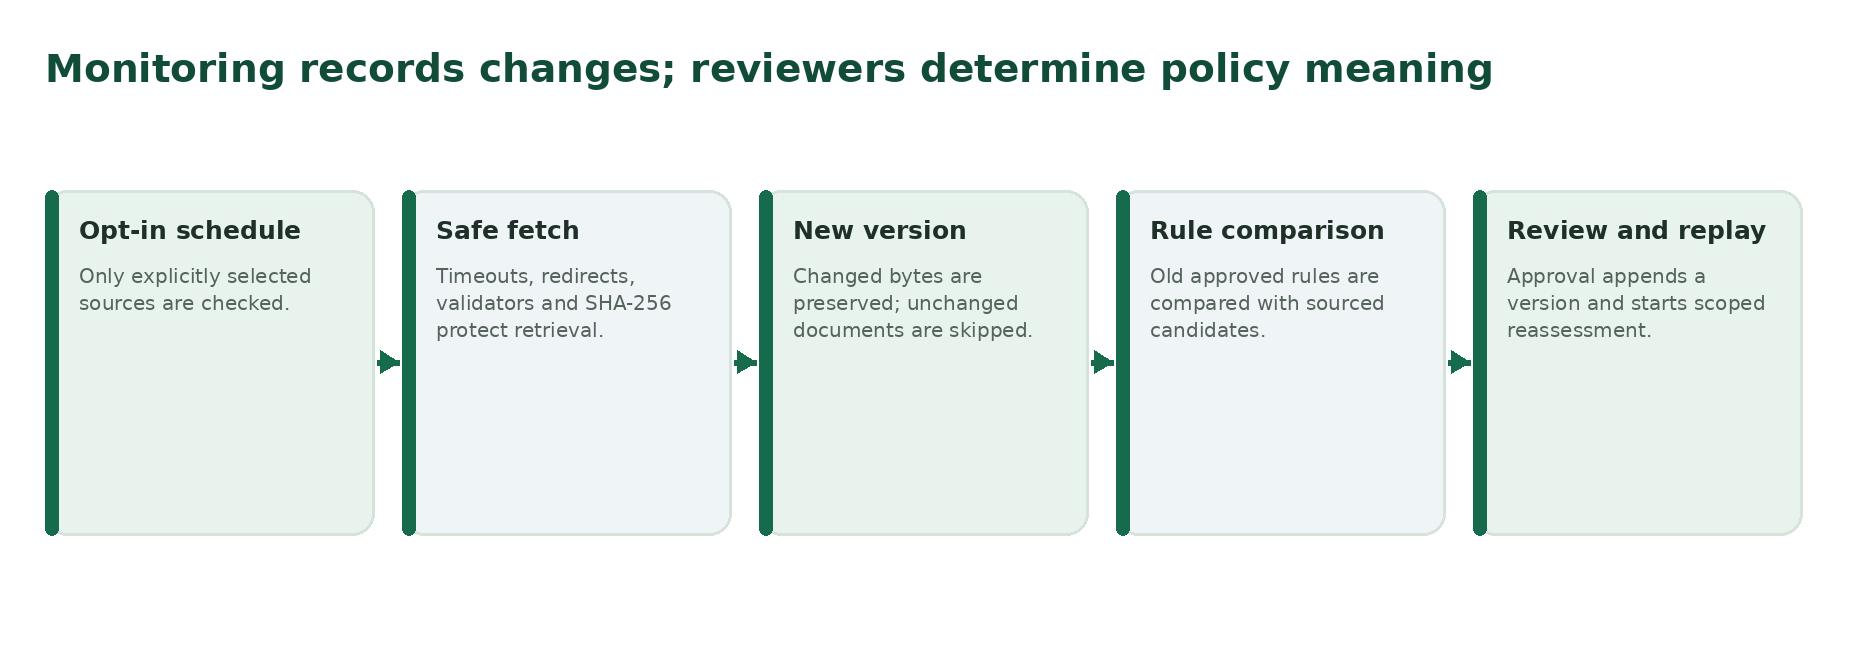
\includegraphics[width=0.94\textwidth,height=0.68\textheight,keepaspectratio]{images/policy-monitoring-workflow.png}\caption{Approved-source monitoring through reassessment}\label{fig:3-3}\end{figure}}{\begin{figure}[htbp]\centering
\resizebox{0.98\textwidth}{!}{%
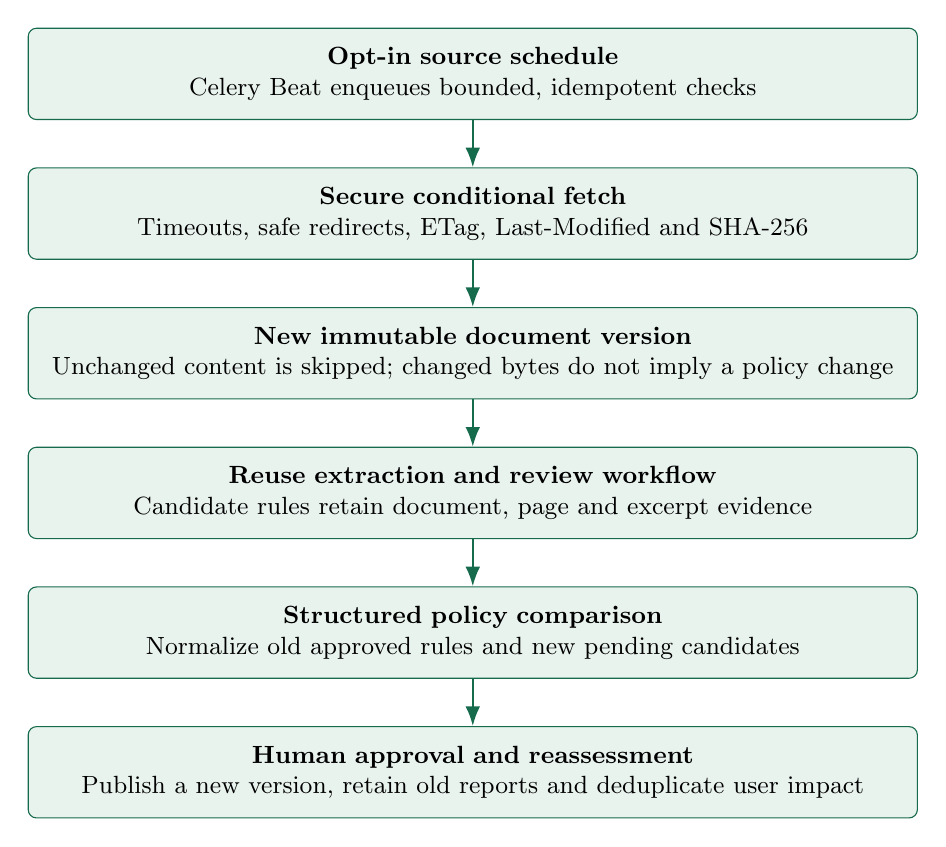
\begin{tikzpicture}[sgbox/.style={draw=sggreen,fill=sglight,rounded corners=3pt,align=center,text width=10.8cm,inner sep=7pt,font=\small},sgarrow/.style={-{Latex[length=2.5mm]},thick,draw=sggreen},node distance=6mm]
\node[sgbox] (n1) {\textbf{Opt-in source schedule}\\Celery Beat enqueues bounded, idempotent checks};
\node[sgbox,below=of n1] (n2) {\textbf{Secure conditional fetch}\\Timeouts, safe redirects, ETag, Last-Modified and SHA-256};
\draw[sgarrow] (n1.south) -- (n2.north);
\node[sgbox,below=of n2] (n3) {\textbf{New immutable document version}\\Unchanged content is skipped; changed bytes do not imply a policy change};
\draw[sgarrow] (n2.south) -- (n3.north);
\node[sgbox,below=of n3] (n4) {\textbf{Reuse extraction and review workflow}\\Candidate rules retain document, page and excerpt evidence};
\draw[sgarrow] (n3.south) -- (n4.north);
\node[sgbox,below=of n4] (n5) {\textbf{Structured policy comparison}\\Normalize old approved rules and new pending candidates};
\draw[sgarrow] (n4.south) -- (n5.north);
\node[sgbox,below=of n5] (n6) {\textbf{Human approval and reassessment}\\Publish a new version, retain old reports and deduplicate user impact};
\draw[sgarrow] (n5.south) -- (n6.north);
\end{tikzpicture}%
}\caption{Approved-source monitoring through reassessment}\label{fig:3-3}\end{figure}}

Administrators opt selected authorized URLs into daily or weekly schedules with access-permission notes and minimum intervals. Celery Beat dispatches durable PostgreSQL jobs; Redis carries their identifiers to bounded workers. ETag and Last-Modified are hints, supplemented by periodic unconditional checksums. An unchanged original does not trigger another model extraction.

Changed bytes create a new DocumentVersion through the existing ingestion service. Normalized text can identify obvious formatting-only changes and avoid a paid call, but cannot prove visual/table equivalence. The source remains inspectable and potentially outdated until the policy situation is resolved.

\subsection*{Structured policy differences}

The comparison engine normalizes typed leaves and compares stable condition identifiers together with their logical context. It detects threshold changes, categorical/state/education changes, exclusions, added or removed conditions and altered expression relationships. Missing proposal clauses are inconclusive until a reviewer establishes completeness. Supported deadline and required-document labels may be compared as source facts without inventing executable operators.

\begingroup\small\renewcommand{\arraystretch}{1.18}
\begin{longtable}{|>{\RaggedRight\arraybackslash}p{0.3600\textwidth}|>{\RaggedRight\arraybackslash}p{0.6000\textwidth}|}
\caption{Change classification and activation behavior}\label{tab:change-classification-and-activation-behavior}\\
\hline\rowcolor{sglight}\textbf{Observation} & \textbf{Classification / action} \\ \hline
\endfirsthead
\caption[]{Change classification and activation behavior (continued)}\\
\hline\rowcolor{sglight}\textbf{Observation} & \textbf{Classification / action} \\ \hline
\endhead
\hline\multicolumn{2}{r}{Continued on next page}\\\endfoot
\hline\endlastfoot
Same original checksum & Unchanged; retain version and skip AI processing. \\ \hline
Different bytes, identical normalized text & Potential formatting change; retain original and allow inspection. \\ \hline
Same typed value, different decimal spelling & Normalized equivalence; do not invent a material threshold change. \\ \hline
Evidence-backed income or age threshold differs & Proposed material change requiring human review. \\ \hline
Missing clause / uncertain table or date & Inconclusive; request clarification, keep prior approved version. \\ \hline
Approved exact revision and valid publication & Publish immutable replacement and queue authorized impact processing. \\ \hline
\end{longtable}
\endgroup\vspace{0.3em}

For example, a \textbf{fictional test policy} changing an income ceiling from INR 250000 to INR 300000 is recorded as a proposed threshold increase with old/new evidence. The numbers are not assigned to any government scheme. Human approval, not the diff classification, activates a new rule.

A failed fetch, unverified document or ambiguous candidate never removes the last approved policy. Currency warnings communicate potential staleness. Public policy-update responses expose only changes linked to verified published rules, while pending proposals stay in the protected administrator workspace.

\section{Reassessment, Notifications and Privacy}

When a material policy change is approved, the publication transaction also records a durable reassessment job. The worker rechecks approval, effective date and whether a later publication already supersedes the queued version. Future-effective changes wait until the applicable date in Asia/Kolkata. Rollback publishes neither a policy nor its reassessment request.

The worker identifies affected saved assessments and locks each active citizen account before reading authorized data. It respects reassessment consent and current notification preferences. Necessary fields come from the current encrypted profile; missing or deleted profile data yields UNKNOWN. The original assessment is never modified.

A new encrypted assessment pins the new approved rule, input snapshot and trace, with links to its parent and policy change. The impact record compares condition-level outcomes. Per-account transactions commit the report, event and notification together. Deterministic identifiers, account locks and unique event keys prevent duplicate effects after a crash or redelivery.

\subsection*{Notification semantics}

In-app messages identify verified policy updates, affected prior assessments, changed conditions, new information requirements or deadline changes. Notifications are owner-scoped, readable/unreadable by the recipient only, and preference-aware. Generic titles avoid exposing sensitive profile details; detailed reports require an authorized session. The application does not send email in the current MVP.

Guest recommendation inputs remain in per-tab React memory and are cleared on reload or session changes. Registered citizens explicitly consent to profile persistence through the existing encrypted store. Historical encrypted assessment snapshots are retained for reproducibility unless the account is deleted through the authorized purge process. Encryption protects sensitive payloads, but operators still control database access, key custody and backup retention.

\clearpage\chapter{System Design and Implementation}

\section{Technology Stack}

SchemeGuard uses a modular Python backend and a typed React frontend. Dependencies are pinned in the repository. The table records the implementation families rather than claiming compatibility with every future release.

\begingroup\small\renewcommand{\arraystretch}{1.18}
\begin{longtable}{|>{\RaggedRight\arraybackslash}p{0.1800\textwidth}|>{\RaggedRight\arraybackslash}p{0.3600\textwidth}|>{\RaggedRight\arraybackslash}p{0.4200\textwidth}|}
\caption{Implemented technology stack}\label{tab:implemented-technology-stack}\\
\hline\rowcolor{sglight}\textbf{Layer} & \textbf{Technologies} & \textbf{Role} \\ \hline
\endfirsthead
\caption[]{Implemented technology stack (continued)}\\
\hline\rowcolor{sglight}\textbf{Layer} & \textbf{Technologies} & \textbf{Role} \\ \hline
\endhead
\hline\multicolumn{3}{r}{Continued on next page}\\\endfoot
\hline\endlastfoot
Interface & Next.js 16, React 19, TypeScript, Tailwind CSS 4 & Responsive pages, forms and server-side API proxies. \\ \hline
API / validation & Python 3.12, FastAPI, Pydantic, pydantic-settings & Typed routes, dependency injection and environment validation. \\ \hline
Persistence & PostgreSQL 16, SQLAlchemy, asyncpg, Alembic, pgvector & Relational history, async sessions, migrations and vectors. \\ \hline
Document / AI & PyMuPDF, Google GenAI SDK, LangGraph & Bounded parsing, candidates and checkpointed review. \\ \hline
Background work & Celery, Redis, Celery Beat & Durable-job delivery, bounded workers and scheduling. \\ \hline
Security / verification & Argon2id, Fernet, pytest, HTTPX, Vitest, Playwright & Credentials, private payloads and regression coverage. \\ \hline
\end{longtable}
\endgroup\vspace{0.3em}

\section{Module Description}

The repository separates HTTP contracts, application services, repositories, schemas and models. Background tasks call existing services rather than duplicating policy processing or decision logic. The frontend reuses the same backend recommendation contract for guests, the saved-profile endpoint and the dashboard.

\begingroup\small\renewcommand{\arraystretch}{1.18}
\begin{longtable}{|>{\RaggedRight\arraybackslash}p{0.3395\textwidth}|>{\RaggedRight\arraybackslash}p{0.6205\textwidth}|}
\caption{Backend modules and responsibility boundaries}\label{tab:backend-modules-and-responsibility-boundaries}\\
\hline\rowcolor{sglight}\textbf{Module / package} & \textbf{Responsibility} \\ \hline
\endfirsthead
\caption[]{Backend modules and responsibility boundaries (continued)}\\
\hline\rowcolor{sglight}\textbf{Module / package} & \textbf{Responsibility} \\ \hline
\endhead
\hline\multicolumn{2}{r}{Continued on next page}\\\endfoot
\hline\endlastfoot
api/v1 + schemas & Versioned endpoints, request/response validation and authorization dependencies. \\ \hline
models + repositories & Canonical relational entities, scoped queries, version selection and transaction boundaries. \\ \hline
services/recommendations & Catalog relevance, explainable factors, filtering and stable pagination. \\ \hline
eligibility & Typed expression validation, normalization, three-valued evaluation and traces. \\ \hline
assessment & Separate project-authored template loading and explicit assessment basis. \\ \hline
ingestion + ai & Official acquisition, parser/storage/chunks, structured extraction and candidate validation. \\ \hline
agents + rag & Checkpointed graph, review/publication orchestration and approved-source retrieval. \\ \hline
services/monitoring + policy\_diff & Opt-in source checks, document comparison and reviewed changes. \\ \hline
workers + services/jobs & Outbox dispatch, leases, retries, locks and durable task execution. \\ \hline
auth + citizen services & Shared role/session infrastructure, encrypted profiles, history and notifications. \\ \hline
\end{longtable}
\endgroup\vspace{0.3em}

Core services depend on typed schemas and repositories; routes remain thin. PostgreSQL is authoritative for policy approval and job state. The same RuleSet, RuleCondition, RuleEvidence and DocumentVersion concepts are retained across all phases, avoiding a parallel AI policy store.

\section{Individual Contributions}

The supplied material identifies Ankesh as the project contact, but does not establish a complete team roster or a verified division of authorship. The report therefore records implemented work packages without assigning unsupported individual credit. Team members should confirm their actual allocations before an assessed submission; the sample report's unrelated author names have not been copied.

\begingroup\small\renewcommand{\arraystretch}{1.18}
\begin{longtable}{|>{\RaggedRight\arraybackslash}p{0.2810\textwidth}|>{\RaggedRight\arraybackslash}p{0.6790\textwidth}|}
\caption{Implemented work packages for contribution review}\label{tab:implemented-work-packages-for-contribution-review}\\
\hline\rowcolor{sglight}\textbf{Work package} & \textbf{Deliverables recorded in the repository} \\ \hline
\endfirsthead
\caption[]{Implemented work packages for contribution review (continued)}\\
\hline\rowcolor{sglight}\textbf{Work package} & \textbf{Deliverables recorded in the repository} \\ \hline
\endhead
\hline\multicolumn{2}{r}{Continued on next page}\\\endfoot
\hline\endlastfoot
Backend and database & FastAPI services, SQLAlchemy models, migrations, transactional seeding and typed APIs. \\ \hline
Eligibility and recommendations & Typed rule engine, version-aware selection, relevance scoring, traces and missing-information behavior. \\ \hline
Document intelligence & Official PDF acquisition, extraction, candidate validation, LangGraph review and source-grounded retrieval. \\ \hline
Citizen and administrator interface & Profile-first discovery, responsive reports, protected workspaces and review/monitoring pages. \\ \hline
Automation and security & Celery/Beat/Redis, reassessment, sessions, encryption, audit and deployment guards. \\ \hline
Quality and documentation & PostgreSQL integration tests, browser journeys, evaluation fixtures, recovery drill and phase reports. \\ \hline
\end{longtable}
\endgroup\vspace{0.3em}

\subsection*{Development process}

The implementation was extended incrementally across seven phases and later profile-first refinements. Each phase preserved existing migrations and records, added focused tests and kept the application runnable through Docker. The later recommendation redesign reused encrypted profiles and strict eligibility rather than replacing either subsystem.

Authorship, supervision and academic approval are institutional facts, not values inferable from code. Signature pages remain unsigned. No project guide name, roll number, institutional logo or degree certification is fabricated from the reference template.

\section{User Interface and Primary Journey}

\IfFileExists{images/profile-first-journey.png}{\begin{figure}[htbp]\centering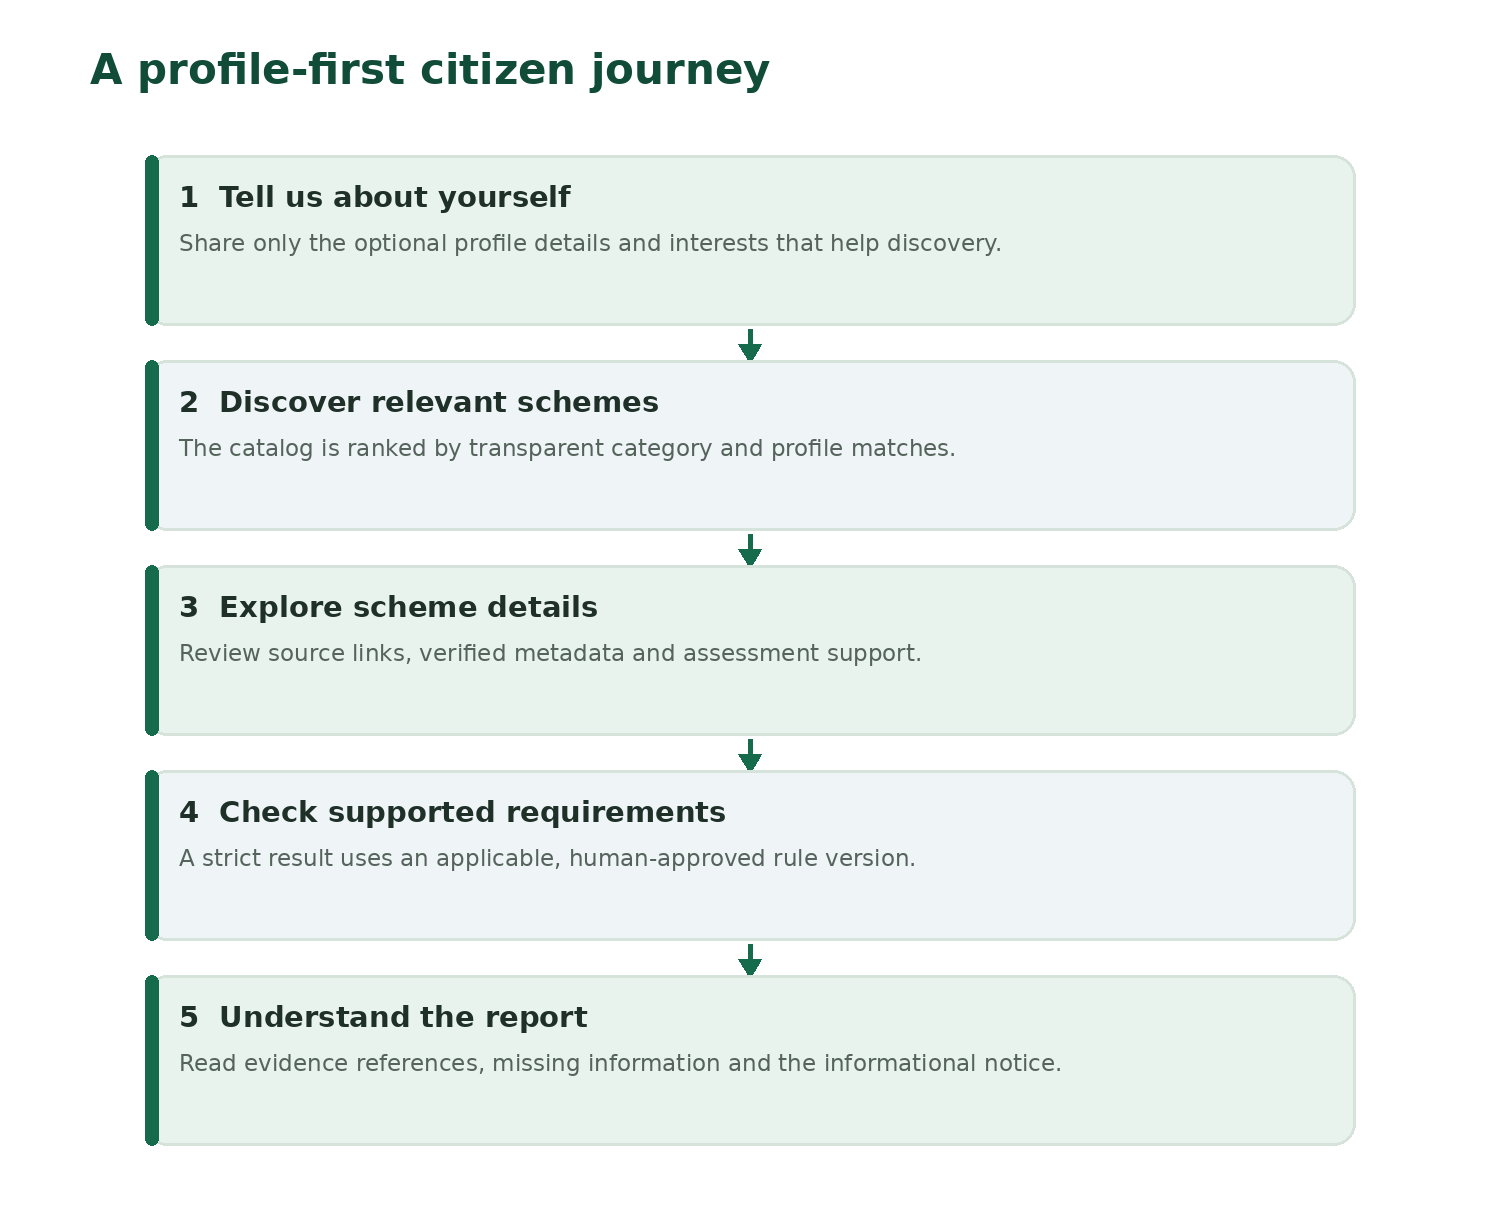
\includegraphics[width=0.94\textwidth,height=0.68\textheight,keepaspectratio]{images/profile-first-journey.png}\caption{Profile-first citizen journey}\label{fig:4-1}\end{figure}}{\begin{figure}[htbp]\centering
\resizebox{0.98\textwidth}{!}{%
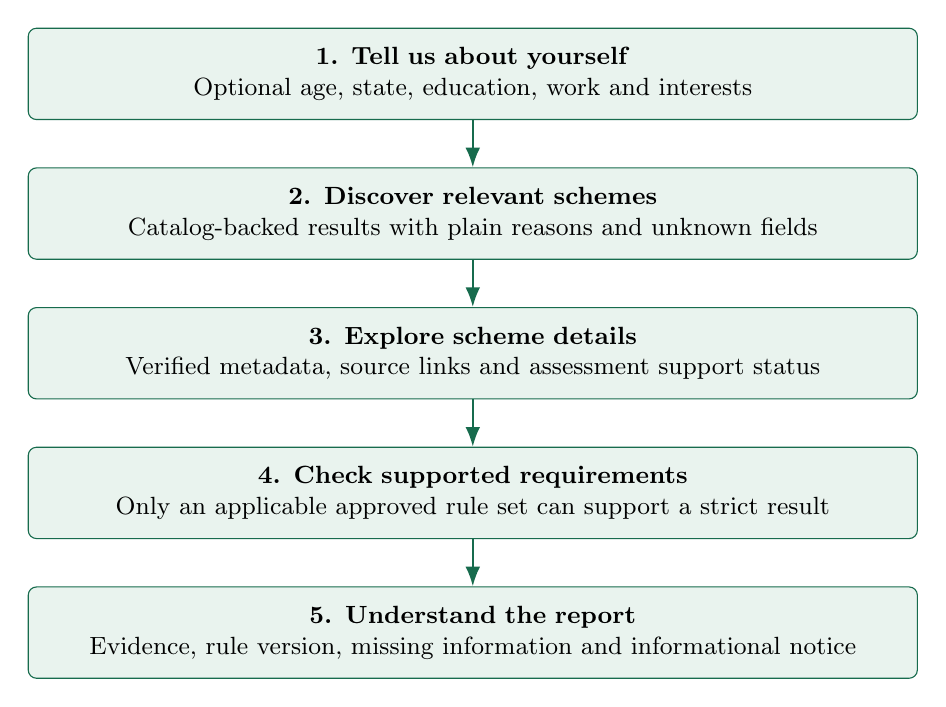
\begin{tikzpicture}[sgbox/.style={draw=sggreen,fill=sglight,rounded corners=3pt,align=center,text width=10.8cm,inner sep=7pt,font=\small},sgarrow/.style={-{Latex[length=2.5mm]},thick,draw=sggreen},node distance=6mm]
\node[sgbox] (n1) {\textbf{1. Tell us about yourself}\\Optional age, state, education, work and interests};
\node[sgbox,below=of n1] (n2) {\textbf{2. Discover relevant schemes}\\Catalog-backed results with plain reasons and unknown fields};
\draw[sgarrow] (n1.south) -- (n2.north);
\node[sgbox,below=of n2] (n3) {\textbf{3. Explore scheme details}\\Verified metadata, source links and assessment support status};
\draw[sgarrow] (n2.south) -- (n3.north);
\node[sgbox,below=of n3] (n4) {\textbf{4. Check supported requirements}\\Only an applicable approved rule set can support a strict result};
\draw[sgarrow] (n3.south) -- (n4.north);
\node[sgbox,below=of n4] (n5) {\textbf{5. Understand the report}\\Evidence, rule version, missing information and informational notice};
\draw[sgarrow] (n4.south) -- (n5.north);
\end{tikzpicture}%
}\caption{Profile-first citizen journey}\label{fig:4-1}\end{figure}}

The landing page prioritizes Find My Schemes and does not load a catalog grid. The five-step questionnaire collects optional age/state, education/student/course information, occupation/employment, family income and interests. Users can skip unknown answers. Names, Aadhaar numbers and identity documents are unnecessary for recommendation.

Personalized results show relevance labels, reasons, missing information, category filters and pagination. Scheme details present verified metadata and an official source link before offering a supported assessment. The report groups passed, failed and unknown requirements and explains its policy basis. Users can return to edit details without repeating unrelated questions.

\subsection*{Implemented result cards and responsive presentation}

\IfFileExists{images/recommendation-cards-desktop.png}{\begin{figure}[htbp]\centering
\includegraphics[width=0.94\textwidth,height=0.68\textheight,keepaspectratio]{images/recommendation-cards-desktop.png}\caption{Schematic of a recommendation card and its explanation}\label{fig:4-2}\end{figure}}{\begin{figure}[htbp]\centering
\resizebox{0.9\textwidth}{!}{%
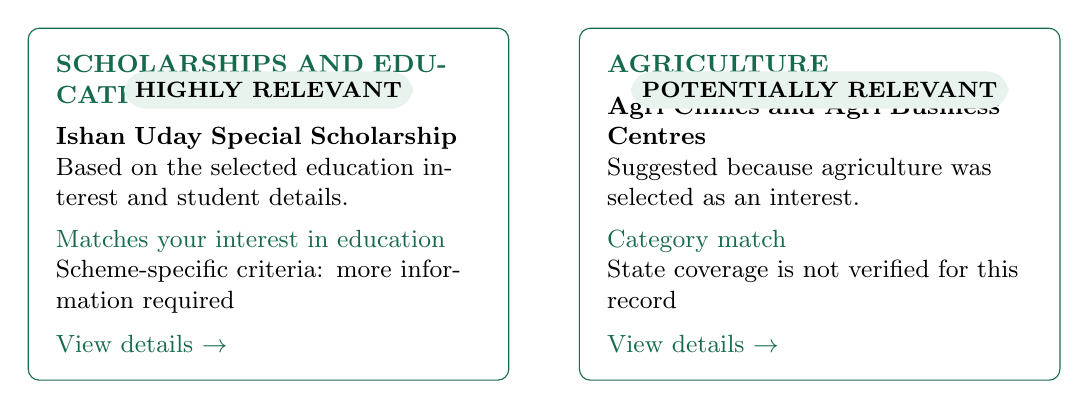
\begin{tikzpicture}[sgbox/.style={draw=sggreen,fill=white,rounded corners=4pt,align=left,text width=5.4cm,minimum height=3.5cm,inner sep=10pt,font=\small},sgtag/.style={fill=sglight,rounded corners=8pt,inner sep=4pt,font=\footnotesize\bfseries}] 
\node[sgbox] (card1) at (0,0) {\textcolor{sggreen}{\textbf{SCHOLARSHIPS AND EDUCATION}}\\[4pt]\textbf{Ishan Uday Special Scholarship}\\Based on the selected education interest and student details.\\[4pt]\textcolor{sggreen}{Matches your interest in education}\\Scheme-specific criteria: more information required\\[5pt]\textcolor{sggreen}{View details $\rightarrow$}};
\node[sgbox] (card2) at (7,0) {\textcolor{sggreen}{\textbf{AGRICULTURE}}\\[4pt]\textbf{Agri Clinics and Agri Business Centres}\\Suggested because agriculture was selected as an interest.\\[4pt]\textcolor{sggreen}{Category match}\\State coverage is not verified for this record\\[5pt]\textcolor{sggreen}{View details $\rightarrow$}};
\node[sgtag] at (0,1.45) {HIGHLY RELEVANT};\node[sgtag] at (7,1.45) {POTENTIALLY RELEVANT};
\end{tikzpicture}%
}\caption{Schematic of a recommendation card and its explanation}\label{fig:4-2}\end{figure}}

The captured cards show the name, category, department, explanation and assessment availability of real catalog records. The source images are archived UI evidence, cropped to the working content area for print; they are not a new browser execution. Matching reasons are explicit rather than a confidence percentage. The displayed illustrative basis must not be mistaken for an approved government policy.

\subsection*{Mobile card detail}

\IfFileExists{images/recommendation-card-mobile.png}{\begin{figure}[htbp]\centering
\includegraphics[width=0.94\textwidth,height=0.68\textheight,keepaspectratio]{images/recommendation-card-mobile.png}\caption{Schematic of the responsive mobile recommendation card}\label{fig:4-3}\end{figure}}{\begin{figure}[htbp]\centering
\resizebox{0.9\textwidth}{!}{%
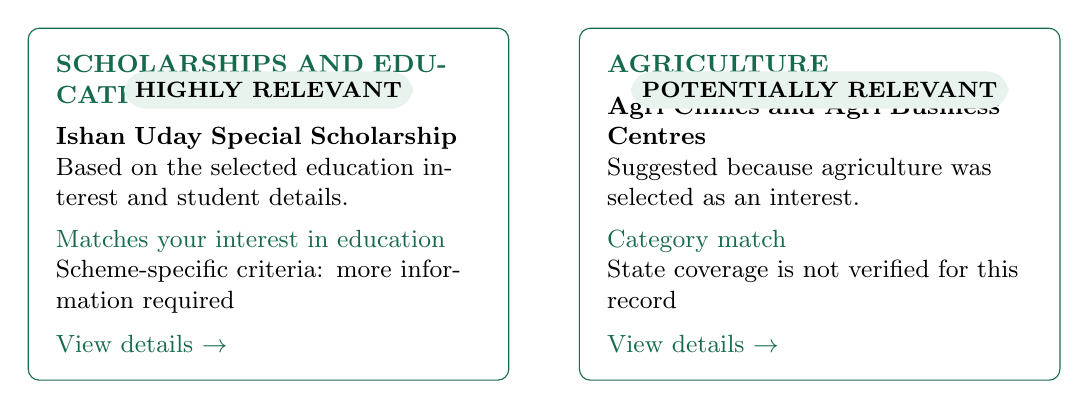
\begin{tikzpicture}[sgbox/.style={draw=sggreen,fill=white,rounded corners=4pt,align=left,text width=5.4cm,minimum height=3.5cm,inner sep=10pt,font=\small},sgtag/.style={fill=sglight,rounded corners=8pt,inner sep=4pt,font=\footnotesize\bfseries}] 
\node[sgbox] (card1) at (0,0) {\textcolor{sggreen}{\textbf{SCHOLARSHIPS AND EDUCATION}}\\[4pt]\textbf{Ishan Uday Special Scholarship}\\Based on the selected education interest and student details.\\[4pt]\textcolor{sggreen}{Matches your interest in education}\\Scheme-specific criteria: more information required\\[5pt]\textcolor{sggreen}{View details $\rightarrow$}};
\node[sgbox] (card2) at (7,0) {\textcolor{sggreen}{\textbf{AGRICULTURE}}\\[4pt]\textbf{Agri Clinics and Agri Business Centres}\\Suggested because agriculture was selected as an interest.\\[4pt]\textcolor{sggreen}{Category match}\\State coverage is not verified for this record\\[5pt]\textcolor{sggreen}{View details $\rightarrow$}};
\node[sgtag] at (0,1.45) {HIGHLY RELEVANT};\node[sgtag] at (7,1.45) {POTENTIALLY RELEVANT};
\end{tikzpicture}%
}\caption{Schematic of the responsive mobile recommendation card}\label{fig:4-3}\end{figure}}

{\small Mobile testing recorded no horizontal overflow at a 390-pixel viewport. The same recommendation contract powers both layouts. Captured catalog descriptions and historical UI content may change independently of the report's verified snapshot. The measured sample counts in Chapter 5 come from the final stored API responses, not from counting screenshot cards.}

\section{Frontend State, Routing and Session Boundaries}

Next.js App Router pages use reusable questionnaire, scheme-card, report, citizen and administrator components. The DiscoveryProvider stores transient answers and explanations only in per-tab memory. Public POST requests go through a fixed same-origin proxy that does not forward account cookies. Personal inputs are not placed in query strings, localStorage, sessionStorage or browser logs.

The routes /find-schemes and /schemes/recommended form the primary discovery experience. /schemes resolves to the questionnaire or personalized results depending on available input; /schemes/all retains manual search and filters. Existing /eligibility routes and saved reports continue to work. Protected layouts check sessions, and backend authorization remains authoritative.

\subsection*{Guests and registered citizens}

Guests can complete discovery and a supported transient assessment without registration. Reloading clears their answers. Registration may carry in-memory answers to an explicit save-consent step, but does not silently store them. Logged-in citizens securely load only their own encrypted profile, can update details and explicitly save changes. Logout, a new login and account deletion clear transient private state.

The dashboard calls the shared recommendation engine and retains profile completeness, saved assessments, notifications and verified policy updates. It no longer relies on geographic suggestions alone. Recently viewed tracking has not been introduced. Incomplete profiles receive a useful prompt; an empty profile produces no unrelated scheme grid.

\subsection*{Interface feedback}

Forms use accessible labels, bounded inputs, clear validation, back/next controls and unknown answers. Pages include loading, error and empty states. Assessment actions are offered only when the server identifies an approved policy or explicit illustrative template. Unsupported schemes display that detailed criteria are not yet available. No public screen can publish extracted policy candidates.

\section{Database Design and Canonical Relationships}

\begin{figure}[htbp]\centering
\resizebox{0.98\textwidth}{!}{%
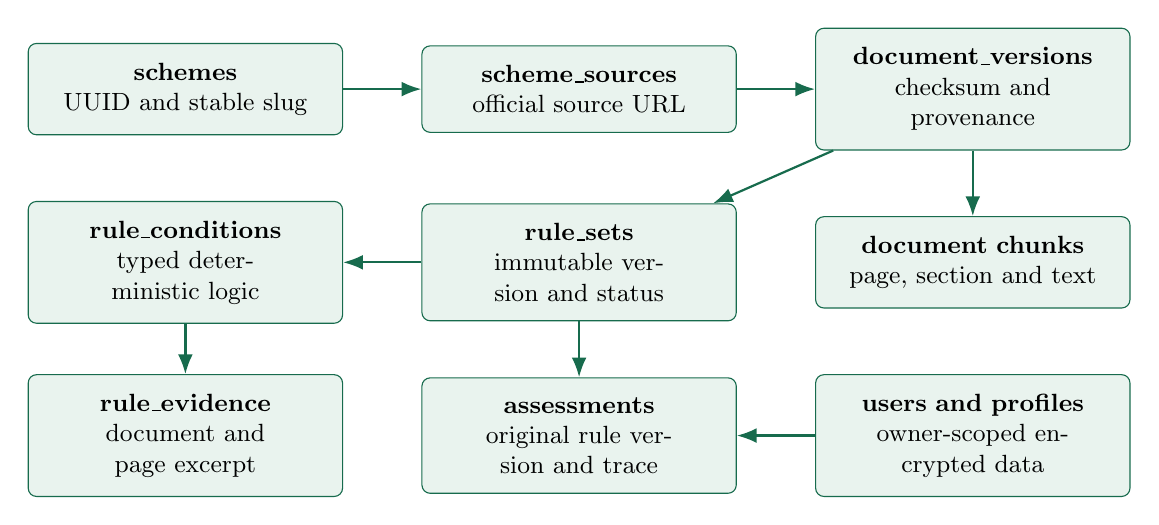
\begin{tikzpicture}[sgbox/.style={draw=sggreen,fill=sglight,rounded corners=3pt,align=center,text width=3.5cm,inner sep=7pt,font=\small},sgarrow/.style={-{Latex[length=2.5mm]},thick,draw=sggreen}] 
\node[sgbox] (s) at (0,0) {\textbf{schemes}\\UUID and stable slug};
\node[sgbox] (src) at (5,0) {\textbf{scheme\_sources}\\official source URL};
\node[sgbox] (doc) at (10,0) {\textbf{document\_versions}\\checksum and provenance};
\node[sgbox] (chunks) at (10,-2.2) {\textbf{document chunks}\\page, section and text};
\node[sgbox] (rules) at (5,-2.2) {\textbf{rule\_sets}\\immutable version and status};
\node[sgbox] (conds) at (0,-2.2) {\textbf{rule\_conditions}\\typed deterministic logic};
\node[sgbox] (evid) at (0,-4.4) {\textbf{rule\_evidence}\\document and page excerpt};
\node[sgbox] (assess) at (5,-4.4) {\textbf{assessments}\\original rule version and trace};
\node[sgbox] (profiles) at (10,-4.4) {\textbf{users and profiles}\\owner-scoped encrypted data};
\draw[sgarrow] (s) -- (src);\draw[sgarrow] (src) -- (doc);\draw[sgarrow] (doc) -- (chunks);
\draw[sgarrow] (doc) -- (rules);\draw[sgarrow] (rules) -- (conds);\draw[sgarrow] (conds) -- (evid);
\draw[sgarrow] (rules) -- (assess);\draw[sgarrow] (profiles) -- (assess);
\end{tikzpicture}%
}

\caption{Core entity relationships and evidence lineage}\label{fig:4-4}\end{figure}

UUID domain identifiers and timezone-aware timestamps support stable relationships. A scheme has multiple sources; a source has immutable document versions; a rule set references the exact source document for that scheme. Conditions carry typed expression JSONB, and their evidence refers to the same document and page. Composite constraints and provenance triggers reject cross-document or cross-scheme bindings.

Private profile and assessment payloads are encrypted, while relational references support owner-scoped querying and reproducible rule selection. Operational tables track mutable job/session state; historical documents, reviewed revisions, decisions and policy contents are append-only. Database-owner privileges remain outside the application's normal protection boundary.

\subsection*{Database table inventory}

\begingroup\small\renewcommand{\arraystretch}{1.18}
\begin{longtable}{|>{\RaggedRight\arraybackslash}p{0.2927\textwidth}|>{\RaggedRight\arraybackslash}p{0.6673\textwidth}|}
\caption{Tables grouped by implemented responsibility}\label{tab:tables-grouped-by-implemented-responsibility}\\
\hline\rowcolor{sglight}\textbf{Group} & \textbf{Tables} \\ \hline
\endfirsthead
\caption[]{Tables grouped by implemented responsibility (continued)}\\
\hline\rowcolor{sglight}\textbf{Group} & \textbf{Tables} \\ \hline
\endhead
\hline\multicolumn{2}{r}{Continued on next page}\\\endfoot
\hline\endlastfoot
Catalog / canonical policy (6) & schemes; scheme\_sources; document\_versions; rule\_sets; rule\_conditions; rule\_evidence. \\ \hline
Authentication / audit (4) & users; login\_sessions; rate\_limits; audit\_events. \\ \hline
Document processing (8) & source\_authorizations; document\_assets; document\_pages; document\_chunks; document\_processing\_jobs; extracted\_rule\_candidates; candidate\_evidence; extraction\_errors. \\ \hline
Workflow / review / retrieval (7) & agent\_workflows; workflow\_events; policy\_reviews; review\_revisions; review\_decisions; rule\_publications; chunk\_embeddings. \\ \hline
Monitoring / durable jobs (6) & background\_jobs; source\_monitoring\_config; monitoring\_runs; policy\_changes; policy\_change\_details; policy\_change\_review\_events. \\ \hline
Citizen private system (5) & profiles; assessments; reassessment\_events; notifications; notification\_preferences. \\ \hline
Migration bookkeeping (1) & public.alembic\_version. \\ \hline
LangGraph checkpoints (4) & sg\_checkpoints.checkpoint\_migrations; checkpoints; checkpoint\_blobs; checkpoint\_writes. \\ \hline
\end{longtable}
\endgroup\vspace{0.3em}

The recorded database has 41 tables including migration/checkpoint bookkeeping [15]. No separate assessment\_conditions table is needed: immutable condition traces and evidence references are stored inside the encrypted saved report, while the exact RuleSet remains relationally linked. Likewise, AI candidates are previews rather than another executable policy representation.

Important constraints include unique scheme slugs, scheme/version uniqueness, deduplicated source document content, stable candidate/page lineage, one active extraction per document, unique publication binding, job deduplication and notification event keys. History triggers prohibit rewriting published content. Indexes support category/state discovery, approved version selection, owner history, unread notifications and dispatch of due jobs.

\section{Incremental Migrations and Data Preservation}

\begingroup\small\renewcommand{\arraystretch}{1.18}
\begin{longtable}{|>{\RaggedRight\arraybackslash}p{0.2576\textwidth}|>{\RaggedRight\arraybackslash}p{0.7024\textwidth}|}
\caption{Applied Alembic revisions and their purpose}\label{tab:applied-alembic-revisions-and-their-purpose}\\
\hline\rowcolor{sglight}\textbf{Revision} & \textbf{Change introduced} \\ \hline
\endfirsthead
\caption[]{Applied Alembic revisions and their purpose (continued)}\\
\hline\rowcolor{sglight}\textbf{Revision} & \textbf{Change introduced} \\ \hline
\endhead
\hline\multicolumn{2}{r}{Continued on next page}\\\endfoot
\hline\endlastfoot
0001\_initial\_metadata & Scheme/source/document tables, UUIDs, constraints and immutable document history. \\ \hline
0002\_eligibility\_rules & Versioned RuleSet, RuleCondition and RuleEvidence; approval/history guards. \\ \hline
0003\_ai\_ingestion & Shared authentication, source authorization, PDF assets/pages/chunks/jobs/candidates/errors. \\ \hline
0004\_least\_privilege & Default new-account role changed to citizen; existing administrators retained. \\ \hline
0005\_workflow\_rag & Review workflow, revisions, decisions, publications, embeddings and pgvector. \\ \hline
0006\_graph\_checkpoints & Versioned PostgreSQL checkpoint schema owned by Alembic. \\ \hline
0007\_workflow\_provenance & Cross-entity integrity and immutable workflow/publication bindings. \\ \hline
0008\_policy\_monitoring & Durable background jobs, source schedules, runs and change history. \\ \hline
0009\_citizen\_system & Encrypted profiles, assessments, preferences, reassessment and notifications. \\ \hline
\end{longtable}
\endgroup\vspace{0.3em}

The recommendation redesign adds optional fields inside the existing encrypted profile JSON and requires no new migration. Older profiles remain valid. The latest recorded Alembic head is 0009\_citizen\_system with no schema drift. New metadata insertion does not overwrite existing slugs or rewrite their source/rule/document history.

Downgrades are tested only in disposable databases. Routine development and releases use forward migrations, retain database/document volumes and back up the encryption key separately. No volume deletion or database reset is part of the documented user journey.

\section{API Design and Integration}

FastAPI provides versioned /api/v1 contracts with Pydantic request and response models. /health reports process liveness; /ready checks PostgreSQL connectivity. UUID parsing, query bounds, controlled error envelopes and request correlation IDs make failures observable without exposing private input. The latest recorded OpenAPI snapshot contains 75 operations [16].

\begingroup\small\renewcommand{\arraystretch}{1.18}
\begin{longtable}{|>{\RaggedRight\arraybackslash}p{0.3817\textwidth}|>{\RaggedRight\arraybackslash}p{0.5783\textwidth}|}
\caption{Representative public and private API contracts}\label{tab:representative-public-and-private-api-contracts}\\
\hline\rowcolor{sglight}\textbf{Method / route} & \textbf{Purpose / boundary} \\ \hline
\endfirsthead
\caption[]{Representative public and private API contracts (continued)}\\
\hline\rowcolor{sglight}\textbf{Method / route} & \textbf{Purpose / boundary} \\ \hline
\endhead
\hline\multicolumn{2}{r}{Continued on next page}\\\endfoot
\hline\endlastfoot
POST /api/v1/recommendations & Transient profile body, relevance ranking, category filter, stable pagination. \\ \hline
GET /api/v1/recommendations/options & Actual catalog category/interest and state choices. \\ \hline
POST /api/v1/me/recommendations & Citizen's own encrypted saved profile; paging options only in body. \\ \hline
GET /api/v1/schemes and /\{id\} & Catalog search, filters, pagination, details and official sources. \\ \hline
POST /api/v1/eligibility/check & Strict approved-policy evaluation; no approved policy means UNKNOWN. \\ \hline
POST /api/v1/assessment/check & Explicit server-selected approved/illustrative/unsupported basis. \\ \hline
GET /api/v1/profiles/me; PUT; DELETE & Owner-only profile management through shared citizen auth. \\ \hline
POST /api/v1/assessments; GET /\{id\} & Save/retrieve private approved-policy reports; reproduce route pins history. \\ \hline
GET /api/v1/notifications & Owner notifications, read actions and preferences on related routes. \\ \hline
POST /api/v1/admin/documents & Administrator-only authorized PDF acquisition and immutable version registration. \\ \hline
\end{longtable}
\endgroup\vspace{0.3em}

The full route inventory is maintained in docs/api.md. Additional administrator groups manage sources, extraction jobs, workflows, review revisions/decisions, indexing, monitors, runs, policy comparisons and audit events. Public policy-updates returns only approved published changes.

\subsection*{Recommendation request and response example}

The request below contains \textbf{synthetic demonstration inputs}. Optional values belong in a POST body, never in a personal-data query string. A guest request does not create a profile or saved assessment.

The recorded request matched 78 schemes, with Ishan Uday Special Scholarship for the North Eastern Region first. Its explanatory factors include the selected education interest, student occupation/status and verified matching geography. Age and income add no ranking points because there is no approved government policy for this record. Assessment availability refers to a separate illustrative basis, not verified government eligibility.

This is an abbreviated shape; actual responses also retain scheme ID, source URL, description, category, missing information and ranking factors. Page size is limited to 30; interests to 24 and free course text to 80 characters. The proxy bounds JSON requests to 16 KB and responses use no-store.

\section{Authentication, Authorization and Private Data}

Citizens and administrators share users, login\_sessions, rate\_limits and audit\_events. Registration always creates a citizen and rejects injected role fields. Administrators are provisioned through an interactive operator command; there is no public admin-registration endpoint. Every private or administrative API checks the active account and required role independently of the frontend.

Passwords use Argon2id with bounded hashing slots. Random opaque session tokens are sent in HttpOnly, SameSite=Strict cookies; only token digests are stored. Production enables Secure cookies. Sessions expire, logout revokes the current token and password changes revoke all sessions. Current-password confirmation protects account changes and deletion. Exact allowed Origin checks and CSRF tokens protect authenticated mutations.

\subsection*{Owner isolation and encryption}

Every private query is scoped to the authenticated owner. Profiles, minimal saved inputs, complete assessment traces and reassessment impacts use authenticated Fernet encryption with owner/purpose binding. Swapped, corrupted or wrong-key payloads fail closed. This is application payload encryption, not whole-database encryption: scheme links, account IDs and overall assessment results remain relational metadata.

PROFILE\_ENCRYPTION\_KEY must remain stable and be shared privately by API and worker. It is not exposed to the frontend or placed in Git. Key rotation requires a deliberate decrypt/re-encrypt migration; simply replacing the key loses access to existing private payloads. Database backups and the separately protected key are both necessary for recovery.

Account deletion purges private profiles, reports, impacts, preferences and notifications, revokes sessions and anonymizes/disables the retained account reference. Policy history and audit integrity remain intact. Profile deletion alone preserves saved historical snapshots for replay. Backup retention/erasure remains an operator responsibility. Email recovery, MFA and verified identity proofing are outside the current implementation.

\section{Application and AI Security Controls}

\begingroup\small\renewcommand{\arraystretch}{1.18}
\begin{longtable}{|>{\RaggedRight\arraybackslash}p{0.2009\textwidth}|>{\RaggedRight\arraybackslash}p{0.4242\textwidth}|>{\RaggedRight\arraybackslash}p{0.3349\textwidth}|}
\caption{Threats, implemented controls and residual limits}\label{tab:threats-implemented-controls-and-residual-limits}\\
\hline\rowcolor{sglight}\textbf{Threat} & \textbf{Implemented control} & \textbf{Residual limit} \\ \hline
\endfirsthead
\caption[]{Threats, implemented controls and residual limits (continued)}\\
\hline\rowcolor{sglight}\textbf{Threat} & \textbf{Implemented control} & \textbf{Residual limit} \\ \hline
\endhead
\hline\multicolumn{3}{r}{Continued on next page}\\\endfoot
\hline\endlastfoot
Cross-user access & Role and owner checks in backend queries; private no-store routes. & A privileged DB operator remains trusted. \\ \hline
Session / CSRF abuse & Hashed revocable sessions, exact Origin, CSRF token, Strict/HttpOnly cookies. & Trusted-edge configuration and MFA remain deployment work. \\ \hline
SSRF / unsafe fetch & Exact official URL authorization, public-IP checks, TLS pinning, no redirects. & Official reachability varies by network. \\ \hline
Malicious PDF & Actual content, size/page/output limits and resource-bounded subprocess. & Not a complete OS sandbox for native parser exploits. \\ \hline
Prompt injection / false rules & Untrusted text, bounded schemas, located evidence and human publication gate. & Reviewers must still resolve semantic ambiguity. \\ \hline
XSS / secret leakage & Escaped text, fixed proxies, production nonce CSP and sanitized logs. & No formal penetration-test certification. \\ \hline
Task duplication / replay & Durable job IDs, locks, leases, terminal checks and uniqueness. & Finite retry exhaustion requires operator intervention. \\ \hline
Historical tampering & Immutable versions, provenance FKs/triggers, revision digests. & Migration owner can bypass database guards. \\ \hline
\end{longtable}
\endgroup\vspace{0.3em}

Request bodies, pagination, expression complexity and costly operations are bounded. SQLAlchemy queries use parameter binding. Request logs retain route, timing, status and correlation ID rather than decrypted applicant inputs or provider keys. Broker tasks contain identifiers only; documents and citizen data are retrieved under service authorization.

The recorded dependency audit reported no known advisories for the checked lockfiles at that time, with no ignore list [19]. This is a dated advisory result, not proof against unknown vulnerabilities or an OS-image scan. Base images, native PDF libraries and SDKs require continued patching and renewed audits before release.

\section{Background Job Reliability and Monitoring}

The backend image serves API, worker and scheduler as separate processes. PostgreSQL background\_jobs is the durable job/outbox authority. Celery uses Redis for JSON-only delivery of job UUIDs. Dispatcher replay can resend a task after a crash; the consumer's database lock, row claim, lease and terminal-state check prevent duplicate business effects. This complements Celery's idempotency guidance [13].

The configured worker concurrency is two, prefetch is one, acknowledgements are late and children recycle after 50 jobs. Soft/hard limits are 420/480 seconds; the durable lease is 600 seconds and broker visibility timeout 900 seconds. Warm shutdown has a nine-minute grace period. Retries are bounded and exponentially delayed rather than infinite.

\subsection*{Scheduling and failure recovery}

Beat dispatches due schedules/outbox work every 30 seconds. A process-lifetime PostgreSQL advisory lock permits one logical scheduler leader. Loss of that connection stops leadership. Per-source daily/weekly UTC schedules and minimum intervals live in PostgreSQL, so changes do not require hardcoded Beat entries.

Transient fetch and provider failures retain durable status and safe error codes. Unsafe destinations and malformed content fail without repeated external access. Expired jobs can be dispatched again, but an active execution lock prevents concurrent processing. A broker outage leaves outbox records available for later delivery. Terminal failures remain visible for investigation.

Monitoring reuses the same secure fetcher, parser, document storage, LangGraph graph and review workflow. A document change does not directly approve policy. Verification failure retains the last approved version and raises a currency warning. Workers do not hot reload backend code; operators restart them after changes while preserving volumes and queued job history.

\section{Docker, Deployment and Observability}

\begin{figure}[htbp]\centering
\resizebox{0.98\textwidth}{!}{%
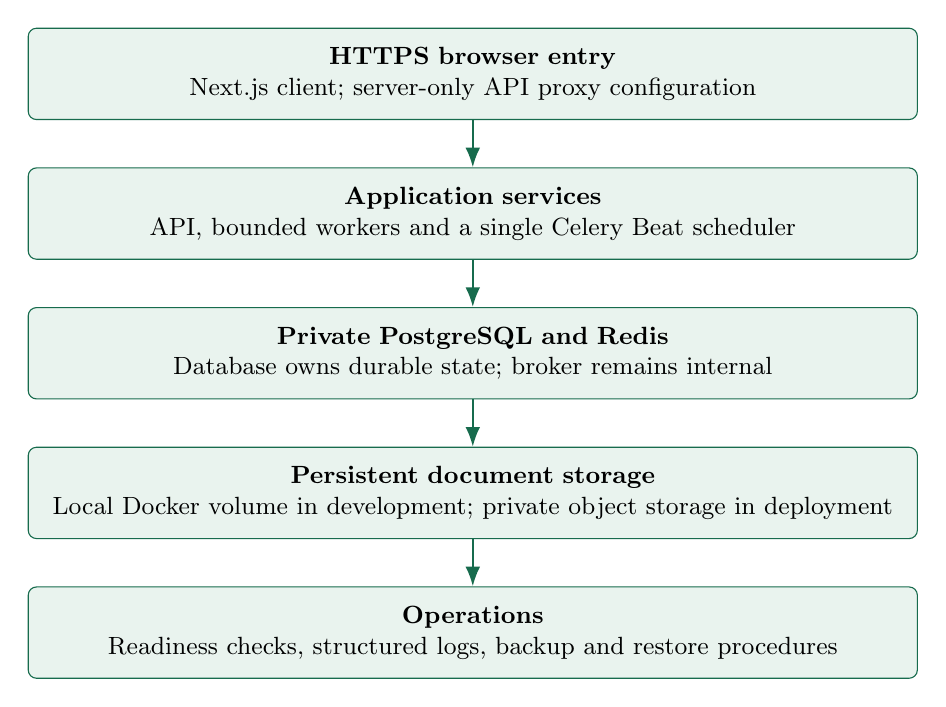
\begin{tikzpicture}[sgbox/.style={draw=sggreen,fill=sglight,rounded corners=3pt,align=center,text width=10.8cm,inner sep=7pt,font=\small},sgarrow/.style={-{Latex[length=2.5mm]},thick,draw=sggreen},node distance=6mm]
\node[sgbox] (n1) {\textbf{HTTPS browser entry}\\Next.js client; server-only API proxy configuration};
\node[sgbox,below=of n1] (n2) {\textbf{Application services}\\API, bounded workers and a single Celery Beat scheduler};
\draw[sgarrow] (n1.south) -- (n2.north);
\node[sgbox,below=of n2] (n3) {\textbf{Private PostgreSQL and Redis}\\Database owns durable state; broker remains internal};
\draw[sgarrow] (n2.south) -- (n3.north);
\node[sgbox,below=of n3] (n4) {\textbf{Persistent document storage}\\Local Docker volume in development; private object storage in deployment};
\draw[sgarrow] (n3.south) -- (n4.north);
\node[sgbox,below=of n4] (n5) {\textbf{Operations}\\Readiness checks, structured logs, backup and restore procedures};
\draw[sgarrow] (n4.south) -- (n5.north);
\end{tikzpicture}%
}

\caption{Production topology and private data services}\label{fig:4-5}\end{figure}

The six-service development configuration is retained. Frontend and API bind loopback ports 3000 and 8000, with database and Redis internal. Named volumes preserve PostgreSQL, originals and broker data. API/frontend hot reload supports development. Production configuration uses separate image targets and Next.js standalone output, non-root application users, health checks, restart/resource/log settings and restricted container permissions.

Production requires a real HTTPS edge, exact frontend origins, stable private keys and reviewed storage/network configuration. The S3 adapter supports private content-addressed originals, but live bucket/IAM connectivity has not been verified. Local production-profile checks used an isolated stack and trusted test certificate; no cloud deployment is claimed.

\subsection*{Service operation and local run commands}

\begingroup\small\renewcommand{\arraystretch}{1.18}
\begin{longtable}{|>{\RaggedRight\arraybackslash}p{0.1636\textwidth}|>{\RaggedRight\arraybackslash}p{0.3382\textwidth}|>{\RaggedRight\arraybackslash}p{0.4582\textwidth}|}
\caption{Docker services and durable responsibilities}\label{tab:docker-services-and-durable-responsibilities}\\
\hline\rowcolor{sglight}\textbf{Service} & \textbf{Function} & \textbf{Readiness / persistence} \\ \hline
\endfirsthead
\caption[]{Docker services and durable responsibilities (continued)}\\
\hline\rowcolor{sglight}\textbf{Service} & \textbf{Function} & \textbf{Readiness / persistence} \\ \hline
\endhead
\hline\multicolumn{3}{r}{Continued on next page}\\\endfoot
\hline\endlastfoot
frontend & Next.js UI and same-origin proxies. & HTTP health; source/dependency volumes in development. \\ \hline
api & FastAPI, shared services and protected contracts. & /ready checks PostgreSQL; persistent document access. \\ \hline
db & PostgreSQL 16 + pgvector. & pg\_isready; named PostgreSQL volume. \\ \hline
redis & Private Celery broker. & Redis health; broker persistence; no host port. \\ \hline
worker & Bounded document/monitor/comparison/reassessment jobs. & Worker liveness and durable PostgreSQL job states. \\ \hline
scheduler & Singleton Beat dispatcher. & Recent heartbeat and PostgreSQL leader lock. \\ \hline
\end{longtable}
\endgroup\vspace{0.3em}

Open the frontend at http://localhost:3000 and API documentation at http://localhost:8000/docs. The government metadata seed is insert-only and repeatable. Demonstration policy seeding is a separate local-development action and must not be treated as government policy onboarding. Never remove persistent volumes to fix an application problem.

Structured logs carry safe request correlation IDs; health/readiness, workflow events, monitoring history, background job failures and audit records provide operational visibility. Logs omit secrets and applicant payloads. GitHub Actions defines lint, type, backend/frontend tests, builds and security checks, but does not automatically deploy production.

\section{Backup, Recovery and Release Procedure}

A complete recovery set includes PostgreSQL public and checkpoint schemas, every referenced original document and the separately retained profile encryption key. Docker volumes provide persistence, not an independent backup. Restricted encrypted backups and explicit retention policies are required. Redis is recoverable delivery state because PostgreSQL retains authoritative jobs.

The repository recovery drill restored a snapshot into a newly generated non-production database, compared table row hashes, verified original PDF checksums and decrypted private sample profiles using the retained key. It did not restore over the working database. A cloud regional failover or managed-storage recovery has not been demonstrated.

\subsection*{Release sequence}

Build immutable reviewed images; execute regression/security checks; back up database, originals and key; validate exact origins and secrets; run one owner-only Alembic upgrade; grant the runtime role only required privileges; start services; verify readiness, sessions, rule history and worker delivery. Enable each source monitor only after access and policy review.

The runtime database role is separate from the migration owner and cannot create schemas, roles or databases. API replicas do not race migrations in the production configuration. A rollback must first confirm schema/job compatibility with the prior image. Prefer a forward corrective migration; do not reverse a publication or rewrite saved reports merely to make an old release start.

\subsection*{Deployment status}

Production Docker images and a local HTTPS production profile were verified in the recorded Phase 7 run. The optional Vercel frontend path is documented but unexecuted. Real DNS/certificates, cloud IAM/storage, managed PostgreSQL/Redis connectivity, secret-manager custody and a reviewed retention policy remain deployment responsibilities. No live cloud resource was created or modified for the report.

\clearpage\chapter{Results and Discussion}

\section{Experimental Setup}

The evaluation uses stored repository verification records rather than a new execution during report preparation. The latest profile-first regression snapshot is dated 14 November 2026 [16]. Backend integration tests use disposable real PostgreSQL databases; frontend tests use Vitest and Testing Library; browser journeys use the project-pinned Playwright runner with isolated installed Chrome.

External government responses and Gemini output are deterministic fixtures in automated AI/monitoring tests. Synthetic citizen profiles and clearly identified fictional policy changes avoid claiming government approval. The A/B/C demonstration executes the actual application services in a disposable database. Human review is simulated against an exact saved revision, not performed by an official authority.

Performance data is local sequential HTTP timing, with warmup excluded and 20 samples per endpoint [18]. Workflow timings are one isolated smoke run, not a load benchmark. No real-model extraction accuracy, independent reviewer agreement, cloud capacity or production SLA is inferred from these tests.

\section{Automated Test Results}

\begingroup\small\renewcommand{\arraystretch}{1.18}
\begin{longtable}{|>{\RaggedRight\arraybackslash}p{0.2560\textwidth}|>{\RaggedRight\arraybackslash}p{0.2773\textwidth}|>{\RaggedRight\arraybackslash}p{0.4267\textwidth}|}
\caption{Latest recorded regression and static verification}\label{tab:latest-recorded-regression-and-static-verification}\\
\hline\rowcolor{sglight}\textbf{Check} & \textbf{Recorded result} & \textbf{Scope} \\ \hline
\endfirsthead
\caption[]{Latest recorded regression and static verification (continued)}\\
\hline\rowcolor{sglight}\textbf{Check} & \textbf{Recorded result} & \textbf{Scope} \\ \hline
\endhead
\hline\multicolumn{3}{r}{Continued on next page}\\\endfoot
\hline\endlastfoot
Backend PostgreSQL regression & 491 passed; 66.61 s & Migrations, engine, API, AI guards, review, monitoring, auth, private data and recommendations. \\ \hline
Frontend unit/component & 84 passed in 13 files; 2.33 s & Forms, result cards, profile/session, admin and error states. \\ \hline
Full browser regression & 9 passed; 35.7 s & Citizen and guest flows, historical reports, manual discovery and authorization. \\ \hline
Final desktop/mobile rerun & 4 passed; 22.8 s & Profile-first journeys at 1280 and 390 pixels. \\ \hline
Python / frontend checks & Passed & Ruff; strict mypy for 109 modules; TypeScript; frontend formatting lint. \\ \hline
Migration drift & None recorded & Head 0009\_citizen\_system; no redesign migration required. \\ \hline
Development / production images & Built & Six development services recorded healthy; production build is not deployment. \\ \hline
\end{longtable}
\endgroup\vspace{0.3em}

The 33 new backend recommendation cases cover category/occupation/student signals, optional income, incomplete inputs, multiple interests, verified and unknown geography, duplicates, ranking, paging, empty results, approved-condition precedence and separation from illustrative thresholds. Guest requests do not write profiles or assessments. Authenticated saved-profile tests verify ownership and CSRF.

Existing regression coverage remains in place for typed comparisons, nested logic, malformed PDFs, unsafe sources, evidence validation, workflow replay, human approval/rejection, policy versions, sessions, cross-user isolation, reassessment and notification deduplication. These are recorded passing runs, not a claim that every possible real-world policy was tested.

\subsection*{Browser journey and privacy observations}

The full primary journey was recorded from the homepage through the optional questionnaire to PostgreSQL-backed recommendations, scheme details, a prefilled supported assessment, report and edit-details return. A citizen run verified saved-profile prefill, explicit encrypted saving, dashboard reuse and logout clearing. Manual browsing, unsupported assessment states and historical report replay remained available.

Browser checks used 1280-pixel desktop and 390-pixel mobile viewports. The final guest run observed zero runtime page errors and zero browser-storage entries. Mobile layout checks found no horizontal overflow in the exercised journey. These are scoped observations, not full assistive-technology certification or every-browser coverage.

\subsection*{Test environment constraints}

The container browser installation encountered mirror/DNS limitations, so the executed local runs used the pinned runner with an isolated installed Chrome. Repeated registration testing reached the existing five-per-hour live throttle. It was preserved rather than disabled. Final repeated citizen checks used a separate temporary QA stack and database; cleanup removed only generated test data through authorized application behavior.

The recorded persistent application remained at 283 schemes, two document versions and the original policy history. Closed generated QA account tombstones were retained by the account deletion design. Such tombstones are audit references, not active citizens. The report avoids presenting mutable personal account counts as a project achievement.

\subsection*{Interpretation}

The browser results substantiate end-to-end wiring and the tested privacy boundaries. They do not prove that all catalog descriptions are current, that a government department will accept an application, or that real model output will always be correct. Those questions require separate policy review and model evaluation.

\section{Recommendation Samples and Ranking Behavior}

\begingroup\small\renewcommand{\arraystretch}{1.18}
\begin{longtable}{|>{\RaggedRight\arraybackslash}p{0.3560\textwidth}|>{\RaggedRight\arraybackslash}p{0.1079\textwidth}|>{\RaggedRight\arraybackslash}p{0.4962\textwidth}|}
\caption{Recorded profile-first API sample outcomes}\label{tab:recorded-profile-first-api-sample-outcomes}\\
\hline\rowcolor{sglight}\textbf{Synthetic input} & \textbf{Matched count} & \textbf{Top recorded result / interpretation} \\ \hline
\endfirsthead
\caption[]{Recorded profile-first API sample outcomes (continued)}\\
\hline\rowcolor{sglight}\textbf{Synthetic input} & \textbf{Matched count} & \textbf{Top recorded result / interpretation} \\ \hline
\endhead
\hline\multicolumn{3}{r}{Continued on next page}\\\endfoot
\hline\endlastfoot
Age 21, Assam, undergraduate student, income INR 240000, education interest & 78 & Ishan Uday Special Scholarship for the North Eastern Region; metadata relevance, not verified eligibility. \\ \hline
Assam and agriculture interest; other inputs unknown & 21 & Agri Clinics and Agri Business Centres ACABC; interest-based relevance. \\ \hline
Unemployed and employment interest & 12 & Capacity Building for Service Providers; employment/skills relevance. \\ \hline
All details unknown & 0 & Useful request for interests or profile details; no unrelated catalog grid. \\ \hline
\end{longtable}
\endgroup\vspace{0.3em}

The student example receives 108 points from the interest, occupation/student and verified geography factors. Age and income contribute zero because no approved government rule exists for the scheme. Missing scheme-specific eligibility conditions remain visible. This demonstrates why relevance and eligibility must not share a label.

The agriculture example confirms that an interest can produce useful discovery without requiring financial or demographic details. The empty-profile case confirms that an unknown profile is not treated as a universal match. State coverage that is unverified remains discoverable, whereas verified incompatibility is filtered explicitly.

These results are captured in profile-first-recommendations-samples.json [16]. They reflect a particular static catalog and input set, not a universal recommendation-quality score. The ranking heuristic has not been validated against independently labeled citizen preferences or real application outcomes. Category metadata may also include institution-oriented programmes; users must inspect official guidance.

\section{End-to-end Policy Workflow Demonstration}

\begingroup\small\renewcommand{\arraystretch}{1.18}
\begin{longtable}{|>{\RaggedRight\arraybackslash}p{0.2890\textwidth}|>{\RaggedRight\arraybackslash}p{0.3200\textwidth}|>{\RaggedRight\arraybackslash}p{0.3510\textwidth}|}
\caption{Isolated synthetic A/B/C integration results}\label{tab:isolated-synthetic-a-b-c-integration-results}\\
\hline\rowcolor{sglight}\textbf{Workflow} & \textbf{Recorded result} & \textbf{Evidence preserved} \\ \hline
\endfirsthead
\caption[]{Isolated synthetic A/B/C integration results (continued)}\\
\hline\rowcolor{sglight}\textbf{Workflow} & \textbf{Recorded result} & \textbf{Evidence preserved} \\ \hline
\endhead
\hline\multicolumn{3}{r}{Continued on next page}\\\endfoot
\hline\endlastfoot
A: document -\textgreater{} extraction -\textgreater{} review -\textgreater{} publication & PASS using PDF and mocked AI; exact-revision human decision simulated. & Original PDF, chunks, candidate evidence, saved review and published version. \\ \hline
B: profile -\textgreater{} discovery -\textgreater{} strict evaluation -\textgreater{} save & PASS in disposable PostgreSQL. & Owner-linked encrypted minimal input, typed trace and original RuleSet. \\ \hline
C: changed PDF -\textgreater{} diff -\textgreater{} new approval -\textgreater{} reassessment & PASS; one deduplicated notification. & Both documents, both approved fixture versions, parent report and impact lineage. \\ \hline
\end{longtable}
\endgroup\vspace{0.3em}

The run preserved two synthetic document versions and two approved fixture rule versions. It confirmed that publication can append new history, the original assessment can still be replayed and duplicate task delivery does not produce duplicate notifications. The database and private fixture data were disposable and rolled back [17].

\subsection*{Real official-document demonstration}

The repository also preserves a historical official Saksham PDF obtained from the National Scholarship Portal. Its previously verified SHA-256 is 06ebed9e50a47ae76cba985ddde78cd65f19f2193b0e4c9c164fff529580474c. Four pages and 26 chunks were recorded, and the original bytes were rechecked in the recovery drill [15].

That document remains pending genuine human policy review and current-guideline reconciliation. It has not produced an approved government RuleSet. A live Gemini run was unavailable in the recorded verification. Therefore the demonstration proves real PDF preservation/parsing and fixture-backed pipeline integration, while live extraction quality and current policy publication remain unverified.

\section{Performance Measurements}

\begingroup\small\renewcommand{\arraystretch}{1.18}
\begin{longtable}{|>{\RaggedRight\arraybackslash}p{0.3757\textwidth}|>{\RaggedRight\arraybackslash}p{0.1252\textwidth}|>{\RaggedRight\arraybackslash}p{0.1461\textwidth}|>{\RaggedRight\arraybackslash}p{0.1461\textwidth}|>{\RaggedRight\arraybackslash}p{0.1670\textwidth}|}
\caption{Recorded local sequential API latency in milliseconds}\label{tab:recorded-local-sequential-api-latency-in-milliseconds}\\
\hline\rowcolor{sglight}\textbf{Endpoint / operation} & \textbf{Samples} & \textbf{Median} & \textbf{p95} & \textbf{Maximum} \\ \hline
\endfirsthead
\caption[]{Recorded local sequential API latency in milliseconds (continued)}\\
\hline\rowcolor{sglight}\textbf{Endpoint / operation} & \textbf{Samples} & \textbf{Median} & \textbf{p95} & \textbf{Maximum} \\ \hline
\endhead
\hline\multicolumn{5}{r}{Continued on next page}\\\endfoot
\hline\endlastfoot
Health & 20 & 2.009 & 2.165 & 2.299 \\ \hline
Database readiness & 20 & 4.742 & 5.267 & 5.318 \\ \hline
Scheme search & 20 & 16.924 & 18.789 & 20.787 \\ \hline
Deterministic assessment & 20 & 18.025 & 19.777 & 19.846 \\ \hline
\end{longtable}
\endgroup\vspace{0.3em}

The measurements used local development Docker services and one sequential client after warmup [18]. They establish responsive behavior for the tested small catalog, not high-concurrency capacity or a service-level objective. Hardware characteristics were not recorded as a controlled benchmark configuration, so cross-machine comparisons would be inappropriate.

\subsection*{Observed query plan}

EXPLAIN ANALYZE recorded a scholarship-name search using a sequential scan followed by a top-N sort. The database query execution was approximately 0.646 ms at the 283-record scale. This is not an observed bottleneck requiring a speculative index. Category/state, approved-version, owner-history, unread-notification and dispatch indexes were reviewed against actual access paths.

\subsection*{Single-run pipeline timings}

The isolated demonstration recorded PDF processing at 426.927 ms, RAG retrieval at 37.561 ms, evaluation-and-save at 39.084 ms, and combined monitor/parse/graph/compare/review at 1255.566 ms. Reassessment was 39.895 ms. Each is one smoke sample, not a percentile or capacity measurement.

Mock extraction took 0.058 ms because no model/network request occurred. It is deliberately excluded from any claim about Gemini speed. Real Gemini, S3, public-government-network latency and heavy PDF concurrency remain unmeasured. Future optimization should be driven by production-like load traces rather than extrapolation from these local samples.

\section{AI Reliability and Decision Evaluation}

A small manually inspected, project-authored reference dataset contains three fictional clauses and 11 boundary/missing-input profiles [17]. The conditions cover an age minimum, an annual income ceiling and a disability-percentage boundary. These values test the engine and evidence guards; they are not government rules. Gold fixture validation is not a measurement of model extraction accuracy.

\begingroup\small\renewcommand{\arraystretch}{1.18}
\begin{longtable}{|>{\RaggedRight\arraybackslash}p{0.2648\textwidth}|>{\RaggedRight\arraybackslash}p{0.2759\textwidth}|>{\RaggedRight\arraybackslash}p{0.4193\textwidth}|}
\caption{Measured fixture evaluation counts and unavailable metrics}\label{tab:measured-fixture-evaluation-counts-and-unavailable-metrics}\\
\hline\rowcolor{sglight}\textbf{Metric} & \textbf{Actual result} & \textbf{Interpretation} \\ \hline
\endfirsthead
\caption[]{Measured fixture evaluation counts and unavailable metrics (continued)}\\
\hline\rowcolor{sglight}\textbf{Metric} & \textbf{Actual result} & \textbf{Interpretation} \\ \hline
\endhead
\hline\multicolumn{3}{r}{Continued on next page}\\\endfoot
\hline\endlastfoot
Located evidence excerpts & 3 / 3 located & Source-location checks on three authored clauses. \\ \hline
Deterministic decisions & 11 / 11 correct & Expected boundary and missing-input outcomes. \\ \hline
False positive eligibility & 0 false PASS among 6 negative cases & Small fixture guard check, not population error rate. \\ \hline
Missing information & 3 / 3 correct & Absent/null fields retained UNKNOWN. \\ \hline
Material change detection & 3 true positives; 0 false positives; 0 false negatives & Precision and recall both 1.0 on this small authored comparison set only. \\ \hline
Live Gemini extraction accuracy & Not measured & No real-model evaluation run available. \\ \hline
Independent human-review agreement & Not measured & No independent annotated reviewer dataset available. \\ \hline
\end{longtable}
\endgroup\vspace{0.3em}

These counts support the correctness of the tested deterministic and evidence checks. They do not justify a claim of 100\% government-policy understanding or universal hallucination resistance. The input set is tiny, hand-authored and not representative of diverse languages, complex exceptions, scanned tables or conflicting departmental amendments.

A future real-model evaluation must use authorized source PDFs, independently annotated complete policies, held-out documents and disagreement analysis. Extraction correctness, evidence correctness, decision correctness and reviewer agreement should be measured separately. No model accuracy percentage is invented in this report.

\section{Security, Persistence and Recovery Results}

The Phase 7 record contains a local HTTPS production-profile smoke test: Secure/HttpOnly cookies, exact CSRF/origin checks, citizen ownership, admin denial and production script nonces were exercised. A runtime database role was verified without superuser, create-database or create-role privileges, and schema DDL was denied. The production worker probe crossed PostgreSQL outbox, singleton Beat, Redis and Celery once; duplicate delivery was skipped [19].

The dependency audit checked 85 pinned Python runtime packages and reported zero known advisories; npm audit reported zero vulnerabilities at that recorded point. Thirty-five browser JavaScript artifacts were scanned for backend-only secret-variable references. These results are dated scope-specific checks, not a current penetration-test certificate or proof against unknown vulnerabilities.

\subsection*{Recovery drill}

The isolated restore recovered 41 tables and 757 snapshot rows into a UUID-named non-production database. Row hashes matched, original PDF checksums were verified and private profiles decrypted with the separately retained key. Only the generated recovery database was removed. This demonstrates the documented local snapshot procedure, not managed-cloud failover or a guaranteed recovery time.

Container recreation checks preserved original documents and public/checkpoint row hashes. The profile-first redesign required no schema migration and retained scheme, source, approved rule and document counts. These checks support data continuity across the tested changes. Backup scheduling, retention, operator access and off-site disaster recovery remain deployment responsibilities.

\subsection*{CI and deployment boundary}

GitHub Actions configuration exists for Python/frontend lint, types, tests, production builds, dependency checks and integration verification. The recorded checks were executed locally; a remote GitHub workflow run and production deployment were not performed. No production credentials are committed and no automatic deployment job is configured.

\section{Discussion and Acceptance Status}

\begingroup\small\renewcommand{\arraystretch}{1.18}
\begin{longtable}{|>{\RaggedRight\arraybackslash}p{0.2538\textwidth}|>{\RaggedRight\arraybackslash}p{0.2759\textwidth}|>{\RaggedRight\arraybackslash}p{0.4303\textwidth}|}
\caption{Completed, demonstrated and unverified functionality}\label{tab:completed-demonstrated-and-unverified-functionality}\\
\hline\rowcolor{sglight}\textbf{Area} & \textbf{Status} & \textbf{Practical meaning} \\ \hline
\endfirsthead
\caption[]{Completed, demonstrated and unverified functionality (continued)}\\
\hline\rowcolor{sglight}\textbf{Area} & \textbf{Status} & \textbf{Practical meaning} \\ \hline
\endhead
\hline\multicolumn{3}{r}{Continued on next page}\\\endfoot
\hline\endlastfoot
Profile-first discovery & Implemented and regression-tested & 282 government metadata records power explainable results. \\ \hline
Strict eligibility engine & Implemented and fixture-tested & Only approved applicable policies execute; government coverage is currently zero. \\ \hline
Official PDF preservation & Real historical PDF processed & Four pages/26 chunks preserved; policy review pending. \\ \hline
Gemini / LangGraph pipeline & Implemented; mocked extraction demonstrated & Live Gemini quality unavailable; approval gate and replay tested. \\ \hline
RAG / review / publication & Fixture integration verified & Approved-version-scoped citations; no broad real-policy benchmark. \\ \hline
Monitoring / reassessment / notifications & Fixture-tested plus real broker probe & No live official sources enrolled in recorded working database. \\ \hline
Docker / security / recovery & Local verification recorded & Production profile tested locally, with no live cloud deployment. \\ \hline
Operational release & Partially prepared & Real credentials, policy onboarding, load tests and cloud controls remain. \\ \hline
\end{longtable}
\endgroup\vspace{0.3em}

The strongest contribution is the controlled connection between modules: recommendations remain separate from policy decisions; AI output stays pending; approved versions retain page evidence; changes append history; saved reports reproduce against their original rule; and task retries cannot silently duplicate effects.

The largest limitation is policy coverage rather than interface breadth. A broad metadata catalog improves discovery but cannot substitute for complete reviewed conditions. The next improvement should prioritize a small, carefully reconciled set of genuine approved policies and independent extraction evaluation before scaling automated processing or claiming real-world benefit outcomes.

\clearpage\chapter{Conclusion and Future Work}

\section{Conclusion}

SchemeGuard implements an integrated academic system for personalized government scheme discovery, evidence-preserving document processing, deterministic eligibility evaluation and reviewed policy change management. It shifts the primary experience from searching a large catalog to providing optional profile information and receiving explainable recommendations.

The architecture keeps three distinct concepts explicit: metadata relevance, project-authored illustrative assessments and human-approved policy execution. The rule engine preserves PASS/FAIL/UNKNOWN semantics, evidence and version-aware reproducibility. Gemini proposes candidates, LangGraph coordinates verification and review, and Celery-based monitoring/reassessment preserves historical originals and reports.

The latest recorded suite passed 491 backend tests, 84 frontend tests and nine browser tests. The catalog contains 282 government discovery records; no government rule set is yet approved. Synthetic workflows demonstrate complete publication, historical replay, change comparison and deduplicated impact notification. These results establish an implemented and tested engineering foundation without claiming official eligibility authority, live model accuracy or production deployment.

\section{Future Work}

\subsection*{Policy coverage and independent evaluation}

Onboard a small set of current official policies with complete page-level evidence, reconciled amendments and genuine reviewer approval. Build an independently annotated, held-out document dataset to measure extraction completeness, citation correctness, false-positive decisions and reviewer agreement. Include complex exceptions, tables and multilingual text before expanding claimed coverage.

\subsection*{Document and monitoring robustness}

Add carefully scoped OCR for selected image-only documents, stronger parser isolation and orphan-blob reconciliation. Evaluate larger PDF collections and realistic network failures. Extend monitoring only to explicitly permitted sources, and add an operator dashboard for exhausted jobs, source-access changes and uncertain policy comparisons.

\subsection*{Privacy and citizen support}

Implement a reviewed retention policy and encryption-key rotation procedure. Add MFA and password recovery only with a verified delivery mechanism. Conduct accessibility testing with assistive technologies and evaluate local-language explanations. Any email notifications must be consent-based and avoid sensitive content.

\subsection*{Deployment and scale}

Verify real HTTPS/cloud storage/IAM, managed database and broker connectivity, off-site backups and restore exercises. Measure realistic concurrent API, parser and reassessment workloads before introducing batch loading, sharding or approximate vector indexes. Preserve explicit publication review and historical replay under every optimization.

Future work should deepen verified policy support and operational confidence rather than turning model fluency or catalog size into an unsupported eligibility claim.

\clearpage\chapter*{References}\addcontentsline{toc}{chapter}{References}\begin{thebibliography}{99}

\bibitem{sgref1}Ministry of Electronics and Information Technology, Government of India. "myScheme." Digital India initiative.\\\url{https://www.digitalindia.gov.in/initiative/myscheme/}

\bibitem{sgref2}Direct Benefit Transfer Mission, Government of India. "Central Scheme List." DBT Bharat. Catalog provenance source; source review recorded 12 November 2026.\\\url{https://dbtbharat.gov.in/central-scheme/list}

\bibitem{sgref3}Government of Goa. "Schemes." Official state government directory. Catalog provenance source; source review recorded 12 November 2026.\\\url{https://www.goa.gov.in/government/schemes/}

\bibitem{sgref4}Government of India. National Scholarship Portal. Official scholarship information and historical scheme guideline source.\\\url{https://scholarships.gov.in/}

\bibitem{sgref5}P. Lewis et al. "Retrieval-Augmented Generation for Knowledge-Intensive NLP Tasks." Advances in Neural Information Processing Systems 33, 2020.\\\url{https://arxiv.org/abs/2005.11401}

\bibitem{sgref6}S. Yao, J. Zhao, D. Yu, N. Du, I. Shafran, K. Narasimhan and Y. Cao. "ReAct: Synergizing Reasoning and Acting in Language Models." ICLR, 2023; arXiv preprint 2022.\\\url{https://arxiv.org/abs/2210.03629}

\bibitem{sgref7}LangChain. LangGraph documentation: interrupts and persistence. Primary implementation reference. Accessed 14 November 2026.\\\url{https://docs.langchain.com/oss/python/langgraph/interrupts}

\bibitem{sgref8}Google. "Structured outputs." Gemini API, Google AI for Developers. Accessed 14 November 2026.\\\url{https://ai.google.dev/gemini-api/docs/structured-output}

\bibitem{sgref9}Artifex Software. "Text." PyMuPDF documentation. Accessed 14 November 2026.\\\url{https://pymupdf.readthedocs.io/en/latest/recipes-text.html}

\bibitem{sgref10}Object Management Group. Decision Model and Notation, version 1.5. Formal specification, 2024.\\\url{https://www.omg.org/spec/DMN/1.5/About-DMN}

\bibitem{sgref11}L. Moreau and P. Missier, editors. PROV-DM: The PROV Data Model. W3C Recommendation, 30 April 2013.\\\url{https://www.w3.org/TR/prov-dm/}

\bibitem{sgref12}OWASP Foundation. "Server Side Request Forgery Prevention Cheat Sheet." OWASP Cheat Sheet Series. Accessed 14 November 2026.\\\url{https://cheatsheetseries.owasp.org/cheatsheets/Server_Side_Request_Forgery_Prevention_Cheat_Sheet.html}

\bibitem{sgref13}Celery Project. "Tasks" and periodic-task documentation. Primary references for acknowledgment, retries and scheduling. Accessed 14 November 2026.\\\url{https://docs.celeryq.dev/en/stable/userguide/tasks.html}

{\small The cited methods and specifications provide context and implementation guidance. SchemeGuard does not claim DMN/PROV certification or reproduction of RAG/ReAct research benchmarks. Government-source citations establish catalog provenance only to the extent stated in the dataset review.}

Repository implementation and verification records

{\small The following are project artifacts, not independent publications. Their recorded results are distinguished from new executions and from external policy authority. Repository: \url{https://github.com/ankesh15/SchemeGuard-AI}.}

\bibitem{sgref14}SchemeGuard repository. docs/datasets.md; backend/app/schemas/seed.py; data/schemes/*.json. Static catalog organization, source review, deduplication and transactional import.

\bibitem{sgref15}SchemeGuard repository. docs/verification/project-facts.json; official-document.json. Recorded catalog/rule/document counts, database table inventory and historical official PDF status.

\bibitem{sgref16}SchemeGuard repository. docs/profile-first-recommendations.md; docs/verification/profile-first-verification.json; profile-first-recommendations-samples.json. Latest recorded user journey, API samples and regression snapshot, 14 November 2026.

\bibitem{sgref17}SchemeGuard repository. docs/verification/demonstration.json; evaluation.json; data/evaluation/phase7.json. Isolated synthetic A/B/C workflows and gold-reference guard/decision evaluation.

\bibitem{sgref18}SchemeGuard repository. docs/verification/performance.json. Local sequential endpoint samples and PostgreSQL query-plan observations.

\bibitem{sgref19}SchemeGuard repository. docs/testing.md; docs/security.md; docs/verification/production.json, production-worker.json, runtime-role.json, recovery.json, dependency-security.json and frontend-bundle.json. Recorded production-profile, security and recovery checks.

{\small Reproducibility note: Paths are relative to the project repository. The report's source package records the document-generation checks separately. Mutable working-database account counts are intentionally not treated as final project metrics.}

\end{thebibliography}\clearpage

\appendix

\clearpage\chapter{Plagiarism and AI-Content Reports}

No institutional plagiarism/similarity report or guide-issued AI-content report was supplied for this document. Consequently, no similarity index, detector score or compliance certificate is claimed. Such reports must be obtained through the institute's authorized process and attached by the submitting authors before final approval.

The reference format includes this appendix. It is retained here as an honest status record rather than filled with a fabricated result. The source template's example threshold is not asserted as a verified requirement of the authors' institute.

\subsection*{Tool-assistance disclosure}

AI assistance was used to organize and draft the report from the supplied reference format and repository records. Programmatic PDF layout and rendering checks were used for formatting. Authors remain responsible for reviewing every technical statement, confirming authorship and supervision details, citing external sources and meeting their institute's academic integrity policy.

\clearpage\chapter{Biographical sketch}

\subsection*{Ankesh}

Ankesh is the project contact identified in the supplied development context for SchemeGuard. The project concerns government scheme discovery, typed eligibility evaluation, document intelligence and policy change management in a full-stack web application.

A verified full author roster, roll numbers, institute, supervisor details, email addresses and educational biography were not provided at report preparation. These personal and institutional facts have therefore not been copied from the unrelated sample report or inferred from a repository username. No CGPA, schooling history or contribution allocation is invented.

This appendix records the available information only. Institutional submission pages require confirmation by the authors and authorized signatories. The editable submission metadata file accompanies the report so confirmed details can be incorporated without rewriting the technical chapters.

\end{document}
